% Options for packages loaded elsewhere
\PassOptionsToPackage{unicode}{hyperref}
\PassOptionsToPackage{hyphens}{url}
%
\documentclass[
]{scrbook}
\usepackage{amsmath,amssymb}
\usepackage{iftex}
\ifPDFTeX
  \usepackage[T1]{fontenc}
  \usepackage[utf8]{inputenc}
  \usepackage{textcomp} % provide euro and other symbols
\else % if luatex or xetex
  \usepackage{unicode-math} % this also loads fontspec
  \defaultfontfeatures{Scale=MatchLowercase}
  \defaultfontfeatures[\rmfamily]{Ligatures=TeX,Scale=1}
\fi
\usepackage{lmodern}
\ifPDFTeX\else
  % xetex/luatex font selection
\fi
% Use upquote if available, for straight quotes in verbatim environments
\IfFileExists{upquote.sty}{\usepackage{upquote}}{}
\IfFileExists{microtype.sty}{% use microtype if available
  \usepackage[]{microtype}
  \UseMicrotypeSet[protrusion]{basicmath} % disable protrusion for tt fonts
}{}
\makeatletter
\@ifundefined{KOMAClassName}{% if non-KOMA class
  \IfFileExists{parskip.sty}{%
    \usepackage{parskip}
  }{% else
    \setlength{\parindent}{0pt}
    \setlength{\parskip}{6pt plus 2pt minus 1pt}}
}{% if KOMA class
  \KOMAoptions{parskip=half}}
\makeatother
\usepackage{xcolor}
\usepackage{longtable,booktabs,array}
\usepackage{calc} % for calculating minipage widths
% Correct order of tables after \paragraph or \subparagraph
\usepackage{etoolbox}
\makeatletter
\patchcmd\longtable{\par}{\if@noskipsec\mbox{}\fi\par}{}{}
\makeatother
% Allow footnotes in longtable head/foot
\IfFileExists{footnotehyper.sty}{\usepackage{footnotehyper}}{\usepackage{footnote}}
\makesavenoteenv{longtable}
\usepackage{graphicx}
\makeatletter
\def\maxwidth{\ifdim\Gin@nat@width>\linewidth\linewidth\else\Gin@nat@width\fi}
\def\maxheight{\ifdim\Gin@nat@height>\textheight\textheight\else\Gin@nat@height\fi}
\makeatother
% Scale images if necessary, so that they will not overflow the page
% margins by default, and it is still possible to overwrite the defaults
% using explicit options in \includegraphics[width, height, ...]{}
\setkeys{Gin}{width=\maxwidth,height=\maxheight,keepaspectratio}
% Set default figure placement to htbp
\makeatletter
\def\fps@figure{htbp}
\makeatother
\setlength{\emergencystretch}{3em} % prevent overfull lines
\providecommand{\tightlist}{%
  \setlength{\itemsep}{0pt}\setlength{\parskip}{0pt}}
\setcounter{secnumdepth}{5}
% definitions for citeproc citations
\NewDocumentCommand\citeproctext{}{}
\NewDocumentCommand\citeproc{mm}{%
  \begingroup\def\citeproctext{#2}\cite{#1}\endgroup}
\makeatletter
 % allow citations to break across lines
 \let\@cite@ofmt\@firstofone
 % avoid brackets around text for \cite:
 \def\@biblabel#1{}
 \def\@cite#1#2{{#1\if@tempswa , #2\fi}}
\makeatother
\newlength{\cslhangindent}
\setlength{\cslhangindent}{1.5em}
\newlength{\csllabelwidth}
\setlength{\csllabelwidth}{3em}
\newenvironment{CSLReferences}[2] % #1 hanging-indent, #2 entry-spacing
 {\begin{list}{}{%
  \setlength{\itemindent}{0pt}
  \setlength{\leftmargin}{0pt}
  \setlength{\parsep}{0pt}
  % turn on hanging indent if param 1 is 1
  \ifodd #1
   \setlength{\leftmargin}{\cslhangindent}
   \setlength{\itemindent}{-1\cslhangindent}
  \fi
  % set entry spacing
  \setlength{\itemsep}{#2\baselineskip}}}
 {\end{list}}
\usepackage{calc}
\newcommand{\CSLBlock}[1]{\hfill\break\parbox[t]{\linewidth}{\strut\ignorespaces#1\strut}}
\newcommand{\CSLLeftMargin}[1]{\parbox[t]{\csllabelwidth}{\strut#1\strut}}
\newcommand{\CSLRightInline}[1]{\parbox[t]{\linewidth - \csllabelwidth}{\strut#1\strut}}
\newcommand{\CSLIndent}[1]{\hspace{\cslhangindent}#1}
\usepackage{booktabs} % for better tables

% fonts
% libertine font: https://www.tug.org/FontCatalogue/linuxlibertine/
\usepackage[oldstyle]{libertine}
\usepackage{libertinust1math}
% \usepackage[T1]{fontenc}
\usepackage[extralight]{inter} 

\usepackage[left=3cm, right=2.5cm, top=2.5cm, bottom=4cm]{geometry} % page margings

\usepackage{tabto} % for aligning text at a certain position, used for title page

\usepackage[ngerman, english]{babel}		% main language is the last in the list, more infor is here: https://en.wikibooks.org/wiki/LaTeX/Internationalization#Babel

\usepackage[onehalfspacing]{setspace}	% clean 1.5 leading / spacing
\RedeclareSectionCommand[beforeskip=1em,afterskip=2em]{chapter} % define space before and after heading

\usepackage{pdfpages} % to include pdfs

% \hypersetup{
% 	unicode=true,          % non-Latin characters in Acrobat’s bookmarks
% 	pdftitle={Rethinking Variation in Social Cognition: Gaze Following across Individuals, Ages, and Communities},    % title
% 	pdfauthor={Julia Christin Prein},     % author
% 	pdfsubject={Dissertation},   % subject of the document
% 	pdfcreator={Julia Christin Prein},   % creator of the document
% 	pdfproducer={Julia Christin Prein}, % producer of the document
% 	pdfkeywords={Social Cognition, Gaze Following, Child Development, Psychometrics, Individual Differences, Cross-cultural Research}, % list of keywords
% 	pdfnewwindow=true,      % links in new PDF window
% 	colorlinks=true,       % false: boxed links; true: colored links
% 	pdfborder={0 0 0},		% color of the border around links
% 	linkbordercolor={0 0 0},
% 	citebordercolor={0 0 0},
% 	urlbordercolor={0 0 0},
% 	linktoc=page,				% defines which part of an entry in the table of contents is made into a link (none,section,page,all)
% 	linkcolor=MidnightBlue,          % color of internal links (change box color with linkbordercolor)
% 	citecolor=MidnightBlue,        % color of links to bibliography
% 	filecolor=MidnightBlue,      % color of file links
% 	urlcolor=MidnightBlue           % color of external links
% }
\ifLuaTeX
  \usepackage{selnolig}  % disable illegal ligatures
\fi
\usepackage{bookmark}
\IfFileExists{xurl.sty}{\usepackage{xurl}}{} % add URL line breaks if available
\urlstyle{same}
\hypersetup{
  hidelinks,
  pdfcreator={LaTeX via pandoc}}

\author{}
\date{\vspace{-2.5em}}

\begin{document}

\frontmatter

\begin{titlepage}                   
    \begin{center}
        
\includegraphics[height=3.2cm]{logo.pdf}\\[40mm]
        
        \huge {\linespread{1.5} Rethinking Variation in Social Cognition: \\ Gaze Following across Individuals, Ages, and Communities}\\[30mm]
        
                
        \normalsize 
        Faculty of Sustainability \\ 
        at Leuphana University Lüneburg\\
        Submitted as a requirement for the award of the title of\\ [10mm]
        
        Doctor of Psychology\\
        -- Dr. rer. nat. --\\[10mm]
        
        Approved dissertation by\\
        Julia Christin Prein\\[10mm]
        
        born February 26, 1995 in Berlin-Kreuzberg, Germany
        
    \vspace*{\fill} 
    \end{center}
    
    \newpage
    \thispagestyle{empty}
    \begin{flushleft}
      \begin{normalsize}
      \vspace*{5mm}
      
            Submitted on: \tabto*{45mm} October 1, 2024 \\
            
            Oral thesis defense on: \tabto*{45mm} February 26, 2025 \\
            
            Year of publication: \tabto*{45mm} 2025 \\[10mm]
            
            First supervisor: \tabto*{45mm} Prof.\,Dr.\, Manuel Bohn, \textit{Leuphana University Lüneburg}\\
                Second supervisor: \tabto*{45mm} Prof.\,Dr.\, Sebastian Wallot, \textit{Leuphana University Lüneburg}\\[5mm]
                First reviewer: \tabto*{45mm} Prof.\,Dr.\, Manuel Bohn, \textit{Leuphana University Lüneburg}\\
                Second reviewer: \tabto*{45mm} Prof.\,Dr.\, Sebastian Wallot, \textit{Leuphana University Lüneburg}\\
                Third reviewer: \tabto*{45mm} Prof.\,Dr.\, Daniel Haun, \textit{Leipzig University \& Max Planck Institute for\\
                \tabto*{45mm} Evolutionary Anthropology Leipzig}\\[10mm]
                
                The individual publications in the cumulative thesis are included in Appendix A of this framework paper and are or will be published as follows: \\[5mm]

Prein, J. C., Kalinke, S., Haun, D. B. M.\*, \& Bohn, M.\* (2024). TANGO: A reliable, open-source, browser-based task to assess individual differences in gaze understanding in 3 to 5-year-old children and adults. *Behavior Research Methods, 56*(3), 2469–2485. \mbox{\url{https://doi.org/10.3758/s13428-023-02159-5}} \\[5mm]

Prein, J. C., Maurits, L., Werwach, A., Haun, D. B. M.,\* \& Bohn, M.\* (2024). Variation in gaze following across the life span: A process-level perspective. *Developmental Science*, Article e13546. \mbox{\url{https://doi.org/10.1111/desc.13546}} \\[5mm]

Bohn, M.\*, Prein, J. C.\*, Ayikoru, A., Bednarski, F. M., Dzabatou, A., Frank, M. C., Henderson, A. M. E., Isabella, J., Kalbitz, J., Kanngiesser, P., Keşşafoğlu, D., Koymen, B., Manrique-Hernandez, M., Magazi, S., Mújica-Manrique, L., Ohlendorf, J., Olaoba, D., Pieters, W., Pope-Caldwell, S., … Haun, D. (2024). *A universal of human social cognition: Children from 17 communities process gaze in similar ways* [Manuscript submitted for publication]. PsyArXiv. \mbox{\url{https://doi.org/10.31234/osf.io/z3ahv}} \\[5mm]

Prein, J. C., Bednarski, F. M., Dzabatou, A., Frank, M. C., Henderson, A. M. E., Kalbitz, J., Kanngiesser, P., Keşşafoğlu, D., Koymen, B., Manrique-Hernandez, M., Magazi, S., Mújica-Manrique, L., Ohlendorf, J., Olaoba, D., Pieters, W., Pope-Caldwell, S., Sen, U., Slocombe, K., Sparks, R. Z., … Bohn, M. (2024). *Measuring variation in gaze following across communities, ages, and individuals – a showcase of the TANGO–CC* [Manuscript submitted for publication]. PsyArxiv. \mbox{\url{https://doi.org/10.31234/osf.io/fcq2g}} \\[10mm]
                
        \end{normalsize}
    \end{flushleft}
    
\end{titlepage}

\chapter{Acknowledgments}\label{acknowledgments}

This dissertation rests on the shoulders of many inspiring, thought-provoking, motivating, and caring individuals. The last four years have been many different things --- but definitely neither boring nor stagnant. I want to thank everyone who has accompanied me on this journey.

My motivation to work on this dissertation is greatly due to my wonderful supervisors, Manuel and Daniel. Manuel, I cannot thank you enough for supporting and believing in me. You have taught me to critically challenge the status quo in research and to focus my energy on improving it --- pragmatically, step by step. Even though I do know that you believe there \emph{are} stupid questions, I felt very comfortable to ask you all along the way and I have benefited a lot from your patience with me. Thanks for roughly 200 meetings that have always left me more motivated and focused than I was before. I cannot imagine how science would be without you! Daniel, I am so happy and proud to have been a member of the CCP team. Thank you for offering me so many unique opportunities and unforgettable memories to travel to conferences and Uganda. I am deeply impressed by how quickly you get a grasp of a new project and know immediately which questions to ask. Thank you for being such an approachable director and having an open door to hear about my personal struggles. To my external supervisor, Robert: your teaching in Research Methods has turned my hate for statistics into a deep passion. Thanks for looking into open PhD positions with me and accompanying me along the way. Without you, I would have never even considered doing a PhD.

Thanks to all the people who made my travels to Uganda so enjoyable. I want to thank the members of the Budongo Families Project, especially Florence, Agnes, Joan and Joseph, for your warm welcome, all your help, hard work and heartfelt laughter.

Thanks to the new people that I met at the Leuphana. Sebastian, thank you for making it possible for me to pursue this doctoral title. Patricia, Franziska, Nele, and (again) Manuel, thanks for the welcoming and kind atmosphere in the LüneLütten lab. I am excited about what is to come next!

I am grateful to our wonderful cohort of PhDs at the MPI. You are a remarkable group of people, and I am very happy that we could share our daily struggles with each other. Noemi, I am so glad that we got to share our office for a (way too short) period of time and successfully solved the Christmas murder mystery with Marie. Wilson, thanks for enduring our laughter through the office walls, for countless lunch breaks together, and for sharing random stories about your fieldwork (and Iceland)! Without my work wife Marie, my time during this dissertation would not have been even half as great as it has been. I could (and have and will) cry thinking about not sharing my daily life with you anymore --- even though I completely trust in our relationship to live until we die. You have made me laugh so much, even if all I wanted to do was cry. Whatever it is that I am up to, I know you will always have my back and help me get back on my feet if I fail. I love your honesty, creativity, immense courage, charming awkwardness, and quirky sense of humor, and feel so honored that you are my friend. Thank you for being you!

My dear, dear family, I am so deeply grateful to know you by my side. Whenever I talk about individual differences, I think about you, Caro, and how we two sisters have the same parents and yet, are so different (in the very best way!!). I believe it is rare that siblings do not feel the need to compete with each other but can just love each other as they are. Thank you! To my mom, who told me right in the beginning that this journey would be a marathon and not a sprint. In some of my darker moments, you told me that even if it felt like I was about to fall, I could never --- because there are so many caring people who would catch me beforehand. Thank you for always having an open home and lots of support (in the form of love, food, vacations, phone calls, and advice) for me. To my dad, thanks for showing up to Leipzig so often and establishing a little concert routine together! I believe I have learned a lot of my problem-solving skills and patience from you. Even if you do not remember saying ``Mach Dinge richtig'' in Caro's and my childhood, I think my dissertation has greatly benefited from this sentence. Thank you, Louis, for helping with my move to Leipzig and spontaneously catching up over coffee in Leipzig or Berlin. To my grandpa, who told me he never worried that I would find my own way. And to my grandma, for all your curiosity, play, and love for children. To Resi and Milou, reminding me to cuddle and catch some fresh air. To the whole Gerken-Prein clan, I could not wish for a better family. Finally, we are reunited in the North.

Thank you to my amazing friends, who constantly remind me to live my life outside the office. To O74, OLAV, and Shubhangi, Schlotti, and Maló, for the cozy home we built together. All our little dance breaks, kitchen karaoke, and reading clubs made even COVID isolatino fun. Thanks for your patience with my mood swings and stealing lunch boxes! Thanks to Laura, for drying my tears, always having an open ear and heart, and helping me with every single move. To Marvin, for all the long hours of deep talk and starting the whole dancing journey with me. To the Kizomba community, especially Carlos and Benedikta, for forcing me to close my eyes, shut off my brain, and relax. Thanks to Arne, for nerding about statistics and providing way too much green mouth refreshener. To the Osna Coxis, especially Merle, Leah, and Alissa, for all the New Year's Eves, regular video calls, big hugs and words of comfort. To Niki, for constantly reaching out, joking around, and asking me how I'm doing. To Ani, Nica, and Schlotti for a lifelong friendship, wholehearted laughter, and a traveling diary. I am so grateful to have every single one of you in my life.

And finally, Steven. You have taken over so many different roles in my life over the last four years. In the beginning, I was simply grateful for your technological support and coding enthusiasm. Thank you for pushing me beyond my levels of comfort and believing in my programming skills (\ldots{} and for being my IT partner ;)). Quickly, however, coding became only one of the thousand topics that we would regularly discuss. Every morning, I looked forward to you making creepy, funny faces on our office door and having long, controversial, and nerdy conversations with you. I deeply miss you in my daily work life. And yet, I do appreciate all the changes that our relationship has gone through in recent years --- through all the highs and lows. I am sincerely grateful and glad to share my life with you. It is so easy being myself around you. Thank you for the commitment, stability, honesty, relaxation, music, joy, and silly jokes that you bring into my life. Your love and support means the world to me. I cannot wait for our new adventures together in Hamburg!

\chapter{Abstract}\label{abstract}

Lorem ipsum dolor sit amet, consectetur adipiscing elit, sed do eiusmod tempor incididunt ut labore et dolore magna aliqua. Luctus venenatis lectus magna fringilla urna. Laoreet non curabitur gravida arcu ac tortor. Faucibus vitae aliquet nec ullamcorper sit amet risus nullam eget. Cras semper auctor neque vitae tempus quam pellentesque. Imperdiet massa tincidunt nunc pulvinar sapien et ligula ullamcorper. Et tortor at risus viverra adipiscing at. Congue nisi vitae suscipit tellus mauris. Habitant morbi tristique senectus et netus et malesuada fames ac. Eget mauris pharetra et ultrices neque. Aenean et tortor at risus viverra. Tempor orci dapibus ultrices in iaculis nunc sed augue. Euismod lacinia at quis risus sed vulputate odio ut enim. Id eu nisl nunc mi ipsum faucibus. Est lorem ipsum dolor sit amet. Eget velit aliquet sagittis id consectetur purus. Faucibus ornare suspendisse sed nisi. Pellentesque diam volutpat commodo sed egestas egestas fringilla.

\chapter{Zusammenfassung}\label{zusammenfassung}

Lorem ipsum dolor sit amet, consectetur adipiscing elit, sed do eiusmod tempor incididunt ut labore et dolore magna aliqua. Luctus venenatis lectus magna fringilla urna. Laoreet non curabitur gravida arcu ac tortor. Faucibus vitae aliquet nec ullamcorper sit amet risus nullam eget. Cras semper auctor neque vitae tempus quam pellentesque. Imperdiet massa tincidunt nunc pulvinar sapien et ligula ullamcorper. Et tortor at risus viverra adipiscing at. Congue nisi vitae suscipit tellus mauris. Habitant morbi tristique senectus et netus et malesuada fames ac. Eget mauris pharetra et ultrices neque. Aenean et tortor at risus viverra. Tempor orci dapibus ultrices in iaculis nunc sed augue. Euismod lacinia at quis risus sed vulputate odio ut enim. Id eu nisl nunc mi ipsum faucibus. Est lorem ipsum dolor sit amet. Eget velit aliquet sagittis id consectetur purus. Faucibus ornare suspendisse sed nisi. Pellentesque diam volutpat commodo sed egestas egestas fringilla.

\renewcommand{\baselinestretch}{1.2}\normalsize
\tableofcontents
\renewcommand{\baselinestretch}{1.5}\normalsize

\chapter{List of Abbreviations}\label{acronyms_HEADER_LOA}

\begin{description}
\tightlist
\item[\phantomsection\label{acronyms_CI}{CI}]
Confidence Interval
\item[\phantomsection\label{acronyms_CLT}{CLT}]
Cross-linguistic Lexical Task
\item[\phantomsection\label{acronyms_CrI}{CrI}]
Credible Interval
\item[\phantomsection\label{acronyms_DISKO}{DISKO}]
Differentiating Incomplete States of Knowledge --- Open
\item[\phantomsection\label{acronyms_FB}{FB}]
False Belief
\item[\phantomsection\label{acronyms_GLMM}{GLMM}]
Generalized Linear Mixed Model
\item[\phantomsection\label{acronyms_IRT}{IRT}]
Item Response Theory
\item[\phantomsection\label{acronyms_PREVIC}{PREVIC}]
Parent Report of Expressive Vocabulary in Children
\item[\phantomsection\label{acronyms_TANGO}{TANGO}]
Task for Assessing iNdividual differences in Gaze understanding --- Open
\item[\phantomsection\label{acronyms_TANGOux2014CC}{TANGO---CC}]
TANGO---Cross-Cultural
\item[\phantomsection\label{acronyms_ToM}{ToM}]
Theory of Mind
\item[\phantomsection\label{acronyms_oREV}{oREV}]
open Receptive Vocabulary task
\end{description}

\chapter*{Authorship Note}\label{authorship}
\addcontentsline{toc}{chapter}{Authorship Note}

In this dissertation, the plural pronoun ``we'' highlights the collaborative efforts within the presented scientific projects. The contributions of all co-authors of the included manuscripts are transparently and accurately attributed using the Contributor Roles Taxonomy (CRediT; \mbox{\url{https://credit.niso.org}}) and can be found for each respective manuscript in \hyperref[appendixA]{Appendix A}. In situations where the primary responsible person is not explicitly defined, ``we'' refers to the efforts of this dissertation's author alone, as the plural pronoun ``we'' reflects standard practice in psychological scientific writings. This use does not diminish the author's significance in conceptualizing, executing, documenting, and interpreting the presented research. The singular pronoun ``I'' explicitly denotes personal opinions, reflections, and decisions regarding this dissertation's theoretical framework paper and its structure.

\chapter*{Structure of this Dissertation}\label{structure}
\addcontentsline{toc}{chapter}{Structure of this Dissertation}

This dissertation is embedded in an overarching, still ongoing project led by Prof.~Dr.~Manuel Bohn (Leuphana University Lüneburg) and Prof.~Dr.~Daniel Haun (Max Planck Institute for Evolutionary Anthropology Leipzig) that will create a new task battery for social cognition. This task battery aims to capture individual differences in children from diverse communities. The present thesis describes the steps that have already been undertaken in this endeavor: during my time as a doctoral candidate, we have designed, implemented, and validated the first task of the battery. We have decided to focus the first task on one of the most fundamental social-cognitive abilities: gaze following.

The present dissertation seeks to approach the development of the new gaze following paradigm from two sides: from a contentual and from a methodological perspective. The first part of the \hyperref[introduction]{Introduction} will focus on the psychological construct(s) underlying gaze following: I will describe the importance of human's social cognition and its milestones during child development. I will continue to elaborate on the construct of gaze following and its developmental milestones. I will end both these sections by considering studies that focus on individual differences and, subsequently, studies that were conducted cross-culturally. The second part of the \hyperref[introduction]{Introduction} will focus on the methodological considerations for constructing a new task battery. I will examine existing social cognition measures, identify common challenges and shortcomings, and establish the need for an individual differences- and cross-cultural research perspective.

The next chapter on the \hyperref[approach]{General Approach} of this dissertation will focus on our aims to develop a new gaze following measure that tackles these recognized methodological challenges. In the \hyperref[discussion]{General Discussion} chapter, I will summarize our study findings, discuss their limitations and provide an outlook for future studies in social cognition, focusing on individual differences and cross-cultural research.

\mainmatter

\chapter{General Introduction}\label{introduction}

Humans share roughly 90 percent of their DNA with that of cats (\citeproc{ref-pontius2007initial}{Pontius et al., 2007}), and even close to 99 percent match our closest living relatives, the chimpanzees (\citeproc{ref-waterson2005initial}{Waterson et al., 2005}). In many ways, we are comparable to other mammals: for example, we have eyes, ears, and noses that sensorily perceive the surroundings, and we have a neocortex that processes this information and performs higher-order brain functions like spatial reasoning and motor commands. In other domains, the animal kingdom far exceeds humans in their abilities and characteristics. Cheetahs can run up to 120 km/h, and Peregrine falcons reach over 380 km/h when diving for prey. Bats and dolphins use echolocation to navigate in complete darkness. Ocean Sunfish have extraordinary reproductive abilities and can lay up to 300 million eggs at once, and the Greenland Shark can live as long as 400 years. So many other species are faster, produce more offspring, and live longer than humans. And yet, the majority of the earth's surface gets populated, exploited, and domesticated by mainly \emph{one} mammal: the \emph{Homo sapiens}. Which abilities brought humans to their ecological success? What makes us uniquely human?

In 1977, NASA launched the Voyager 1 and 2 spacecraft with a golden time capsule as a bold interstellar greeting. This Golden Record aimed to present the essence of Earth and humanity to potential extraterrestrial receivers. It included natural sounds, a selection of music from different cultures, greetings in 55 languages, and a photographic gallery. Among several pictures of mathematical formulas, scientific diagrams and planetary constellations, a large proportion of the included photos focused on the most fundamental human experiences. These pictures showed humans hunting and playing music together, eating and arguing at a full dinner table, collaboratively rowing a boat, competitively running against each other in marathons, nursing their children, and teaching them how to write. Strikingly, humans were rarely presented alone. These photographs, attempting to capture a comprehensive snapshot of Earth's environment, focused on humans interacting with each other in social and cultural groups.

Our ability to engage in social interactions and communicate with others has also been highlighted in prominent evolutionary and psychological theories (e.g., \citeproc{ref-tomasello2019becoming}{Tomasello, 2019}; \citeproc{ref-tomasello2003makes}{Tomasello \& Rakoczy, 2003}). The number of publications in different psychological domains highlights that many psychologists agree on the importance of social cognition. A quick search on the APA PsycNet (on June 25, 2024, at 17:00 CET) revealed 28,594 results for the search term ``social cognition'', while only 3,095 results appeared for ``spatial cognition'' and 95 appeared for ``physical cognition''. Humans have been described as ``ultra-social primates'' (\citeproc{ref-grossmann2022becoming}{Grossmann, 2022, p. 1}). We form social bonds (e.g., \citeproc{ref-bowlby1958nature}{Bowlby, 1958}), live (mostly) cooperatively (e.g., \citeproc{ref-tomasello2020adaptivea}{Tomasello, 2020}), exchange information and learn through observing others (e.g., \citeproc{ref-csibra2009natural}{Csibra \& Gergely, 2009}). By relying on these strategies, knowledge and skills could be passed on from generation to generation --- which could not have possibly been acquired by one single individual (\citeproc{ref-henrich2015secreta}{Henrich, 2015}). Sociality --- and the cognitive abilities enabling it --- might very well be human's superpower.

A seminal paper by Herrmann et al. (\citeproc{ref-herrmann2007humansa}{2007}) tested the hypothesis that humans have unparalleled social-cognitive abilities. The researchers administered a cognitive test battery with 16 different tasks to chimpanzees, orangutans, and 2.5-year-old human infants. Indeed, the results showed that all three groups showed similar cognitive abilities within the physical world (space, quantities, causality), while human infants outperformed the chimpanzees and orangutans when it came to the social world (social learning, communication, Theory of Mind). This study clearly underlines humans' remarkable abilities in the social realm.

\section{Social Cognition}\label{social-cognition}

\subsection{Terminology}\label{terminology}

So far, I have argued for the importance of human's social-cognitive abilities. Before going deeper into the developmental literature on social cognition, let us clarify the term: What is social cognition? Interestingly, there is not one agreed-upon definition accepted by most psychologists. Rather, cynical tongues might say that there are as many definitions of social cognition as there are research articles on it. As Ostrom put it in the Foreword of the Handbook of Social Cognition: ``I regard single-sentence definitions of social cognition to be slightly offensive {[}\ldots{]}. It would be more accurate to say that my preferred definition is the entire Handbook of Social Cognition, both this and the first edition combined.'' (\citeproc{ref-ostrom1994foreword}{Ostrom, 1994, p. vii}). Indeed, researchers have argued that the non-specific and heterogeneous vocabulary hinders empirical and theoretical advancement: sometimes, a single concept is described by several different labels (convergence of meaning), while other concepts share the same label but refer to different constructs (divergence of meaning) (\citeproc{ref-quesque2024defining}{Quesque et al., 2024}; \citeproc{ref-quesque2020theoryofmind}{Quesque \& Rossetti, 2020}).

To get a clearer grasp on what developmental psychologists understand under the term social cognition, we conducted a short expert survey at the beginning of my Ph.D.~(in Autumn/Winter 2020). We distributed an online questionnaire via personal contacts and emailing lists (e.g.~cogdevsoc mailing list) to researchers broadly working in cognitive, comparative, cross-cultural and/or developmental psychology. Out of the 100 experts that completed the survey, more than half held a professorship, and the majority focused on basic research with children. First, we asked experts to define social cognition as a psychological construct. Exactly one third of the sample (33\%, n = 33) chose a definition by Glynn \& Watkiss (\citeproc{ref-glynn2016social}{2016}): ``Social cognition is the process by which actors, at individual or collective levels, decode and encode their social world, using mental models, knowledge structures and cultural understandings to process information, extract meaning and determine appropriate action.'' (p.~1). The next two most frequently chosen definitions focused similarly on the information processing aspects in environments with other agents (``{[}\ldots{]} encompasses all the information-processing mechanisms that underlie how people capture, process, store, and apply information about others to navigate social situations'' (\citeproc{ref-decety2020preface}{Decety, 2020, p. ix}); ``{[}\ldots{]} is concerned with the study of the thought processes, both implicit and explicit, through which humans attain understanding of self, others, and their environment'' (\citeproc{ref-moskowitz2013social}{Moskowitz, 2013, p. 1})). In the next step, we asked experts to name which dimensions they mentioned most often when discussing or writing about social cognition. The dimensions that were chosen by more than half of the experts were beliefs, knowledge, perspective-taking and intentions. Finally, we compiled a list of 21 social-cognitive abilities and asked experts to rate the likelihood that children of the same age would vary to perform these abilities. The experts assumed that children varied mostly in whether they manipulate emotions, deceive others, simulate others' reasoning processes, take another's perspective, and understand the subjectivity of knowledge states. Abilities that were assumed to vary the least between children of the same age were recognizing agents and following gaze. It appeared that experts assumed variation in many social-cognitive abilities and judged the more room for individual differences, the more complex a given social-cognitive ability. Please note that more information on the expert survey can be found in {[}Appendix C{]}.

A related term to social cognition is \hyperref[acronyms_ToM]{Theory of Mind (ToM)}. While these terms are sometimes used synonymously, social cognition functions as the umbrella term that encompasses \hyperref[acronyms_ToM]{ToM}. \hyperref[acronyms_ToM]{ToM} itself describes a system organized around beliefs, desires, and actions that we use in order to make sense of other agents. We try to understand actions by attributing mental states to ourselves and others --- summarized by Wellman as follows: ``in our everyday thinking we construe people as engaging in acts they \emph{think} will get them what they \emph{want}'' (\citeproc{ref-wellman2013universal}{Wellman, 2013, p. 69}). Two characteristics of \hyperref[acronyms_ToM]{ToM} are understanding that mental states are representational (\emph{i.e.,} hold information independent of the real world) and person-specific (\emph{i.e.,} mental states belong to an individual person) (\citeproc{ref-heise2023psychometric}{Heise, 2023}). \hyperref[acronyms_ToM]{ToM} has been traditionally viewed as a unitary construct, but recent neurophysiological evidence suggests a multidimensional structure (\citeproc{ref-fu2023systematicb}{Fu et al., 2023}; \citeproc{ref-slaughter2003introduction}{Slaughter \& Repacholi, 2003}).

\subsection{Developmental Milestones}\label{developmental-milestones}

Importantly, human infants do not come into the world already possessing all these social-cognitive abilities (\citeproc{ref-tomasello2020adaptivea}{Tomasello, 2020}). Much of the developmental psychology research today focuses on how children acquire the social-cognitive abilities needed to become full members of our society.

\begin{itemize}
\tightlist
\item
  developmental milestones in social cognition anreißen
\end{itemize}

\subsection{Individual Differences}\label{individual-differences}

Many decades of research in social cognition have taught us much about developmental milestones and at which average children possess certain social-cognitive abilities (for a review, see \citeproc{ref-rakoczy2022foundations}{Rakoczy, 2022}). For example, we have learned that children are around four to five year of age when they understand that other agents can have false beliefs that differ from the child's own belief and from reality (\citeproc{ref-wellman2001metaanalysis}{Wellman et al., 2001}).

Anyone who has ever interacted with children of a similar age must have noticed that they can still differ in their abilities: some children might be faster in learning how to walk, while others might be quicker in learning how to talk.

\emph{Individual differences} describe the features in which agents vary (``traits or other characteristics by which individuals may be distinguished from one another'', (\citeproc{ref-americanpsychologicalassociationindividual}{American Psychological Association, n.d.-a})). \emph{Inter}-individual differences focus on the variability \emph{between} children, while \emph{intra}-individual differences focus on the variability \emph{within} the same child. Asendorpf (\citeproc{ref-asendorpf1992stability}{1992}) have argued that inter-individual differences are often interpreted as trait-like characteristics (e.g.~personality) that are more or less stable over time, while intra-individual differences might capture state-like characteristics (e.g.~motivation) or development within a given construct. The present thesis and the associated publications focus on inter-individual differences, often abbreviated to individual differences.

A prominent framework that could explain differences between individuals is Vygotsky's sociocultural theory of cognitive development (\citeproc{ref-vygotsky1962thought}{Vygotsky, 1962}, \citeproc{ref-vygotsky1978mind}{1978}, \citeproc{ref-vygotsky1987thinking}{1987}). This theory emphasizes the role of social interaction in children's cognitive development and as such, learning as a social process. In other words, it is assumed that social interaction shapes social cognition.

In order to empirically test if social interaction shapes social cognition, we need to study children's daily environments and cognitive abilities on the individual level.

Studies focusing on individual differences aim to measure variation between children in a given social-cognitive ability and, potentially, study the co-development of certain cognitive abilities or link this variation to internal and external factors that influence its development. As such, individual differences studies act as a powerful tool to build and test developmental theories and the structure of social cognition (\citeproc{ref-happe2017structure}{Happé et al., 2017}). Additionally, individual differences studies are needed to design (clinical or educational) intervention programs. Capturing change before and after an intervention helps to evaluate its efficacy.

\begin{itemize}
\tightlist
\item
  also for modeling, understanding underlying processes?
\end{itemize}

Examples include studies conducted with twins (\citeproc{ref-hughes2005originsa}{Hughes et al., 2005}; \citeproc{ref-ronald2006individual}{Ronald et al., 2006}).

\begin{itemize}
\tightlist
\item
  example from comparative work: some researchers focus on what chimps in average do, others focus on the very end of the distribution: what are they capable of?
\item
  cross-cultural variation: not only average from small samples
\end{itemize}

False-belief understanding can predict children's pretense use, abilities for social interaction, peer popularity, which clearly underlines the relevance of individual differences in social-cognitive abilities for real-life outcomes (\citeproc{ref-wellman2013universal}{Wellman, 2013}).

\subsection{Cross-Cultural Research}\label{cross-cultural-research}

Wellman (\citeproc{ref-wellman2013universal}{2013}) has argued that children's social-cognitive development is a particularly informative domain to assess in which ways people all over the world resemble an differ from one another.

\section{Gaze Following}\label{gaze-following}

\begin{itemize}
\tightlist
\item
  cooperative eye hypothesis
\end{itemize}

\subsection{Terminology}\label{terminology-1}

\subsection{Developmental Milestones}\label{developmental-milestones-1}

\subsection{Individual Differences}\label{individual-differences-1}

\subsection{Cross-Cultural Research}\label{cross-cultural-research-1}

\subsection{Research Gaps}\label{research-gaps}

\section{Methodological Considerations}\label{methodological-considerations}

\subsection{Terminology}\label{terminology-2}

In the context of this work, the terms \emph{variability}, \emph{variation} and \emph{variance} need further explanation. According to the APA Dictionary of Psychology, the definitions of variability and variation greatly resemble each other (variability: ``1. the quality of being subject to change or variation in behavior or emotion, 2. the degree to which members of a group or population differ from each other, as measured by statistics such as the range, standard deviation, and variance'' (\citeproc{ref-americanpsychologicalassociationvariability}{American Psychological Association, n.d.-d}); variation: ``1. the existence of qualitative differences in form, structure, behavior, and physiology among the individuals of a population, whether due to heredity or to environment. Both artificial selection and natural selection operate on variations among organisms, but only genetic variation is transmitted to offspring. 2. in statistics, the degree of variance or dispersion of values that is obtained for a specific variable'' (\citeproc{ref-americanpsychologicalassociationvariation}{American Psychological Association, n.d.-f})). Both definitions focus on differences between individuals that can be applied to the behavioral level. As in most of the developmental literature, the terms variability and variation will be used interchangeably in this work.

As the definitions of variability and variation indicate, the term \emph{variance} denotes a statistical measure for the degree to which group members differ from one another. It describes the dispersion of a distribution by calculating how far the values of a sample spread out from their average value. Consequently, a smaller variance means less differences between individuals in a given sample (``a measure of the spread, or dispersion, of scores within a sample or population, whereby a small variance indicates highly similar scores, all close to the sample mean, and a large variance indicates more scores at a greater distance from the mean and possibly spread over a larger range'', (\citeproc{ref-americanpsychologicalassociationvariance}{American Psychological Association, n.d.-e})).

Psychometric properties of a task are often assessed by its \emph{validity} and \emph{reliability}. \emph{Validity} concerns the truthfulness of a task or the degree to which a task captures what it is designed to measure conceptually (``1. the characteristic of being founded on truth, accuracy, fact, or law. 2. the degree to which empirical evidence and theoretical rationales support the adequacy and appropriateness of conclusions drawn from some form of assessment {[}\ldots{]}'', (\citeproc{ref-americanpsychologicalassociationvalidity}{American Psychological Association, n.d.-c})). There are several different types of validity. In the context of this work, we focus on \emph{convergent} validity (\emph{i.e.,} the degree to which two tasks that should be theoretically related are indeed related), \emph{predictive} validity (\emph{i.e.,} the degree to which a task relates to other tasks separated by a determined period (= predicting scores in the other task)), and \emph{external} validity (\emph{i.e.,} the degree to which the results of a task can be generalized beyond the original sample).

\emph{Reliability} refers to the degree to which a task produces consistent, stable results when repeated again (``the trustworthiness or consistency of a task, that is, the degree to which a test or other measurement instrument is free of random error, yielding the same results across multiple applications to the same sample'', (\citeproc{ref-americanpsychologicalassociationreliability}{American Psychological Association, n.d.-b}); ``). Two main types of reliability are often assessed when evaluating a given task. \emph{Internal consistency} focuses on the relationship between items in the same task to ensure they measure the same construct. \emph{(Test-) Retest reliability} assesses a task's stability over time and estimates the relationship of the task scores on two different administration occasions (e.g., test day one followed by test day two three weeks later).

\subsection{Existing Social Cognition Tasks}\label{existing-social-cognition-tasks}

While a vast variety of social cognition and \hyperref[acronyms_ToM]{ToM} tasks exist, there are not too many that are designed to capture individual differences in children.

Many developmental study paradigms present children with two objects. For example, the Sally-Anne \hyperref[acronyms_FB]{False Belief (FB)} task {[}todo refs{]} lets children witness how a ball gets moved from one box to a basket while another agent does or does not witness the change of location. Children then get asked where the agent believes the ball to be. Possible responses are (1) the box or (2) the basket. Similarly, in the traditional gaze following paradigm {[}todo refs{]}, an agent gazes at a toy to her left- or right-hand side. Common outcome measures focus on children's looking or reaching behavior toward the two toys. What becomes apparent is that these common social cognition tasks rely on dichotomous tasks: a child can either pass or fail the task. Average scores are then calculated (e.g., group level mean), often based on low trial numbers and small sample sizes.

An example to illustrate this point is a longitudinal study by Sodian et al. (\citeproc{ref-sodian2016understanding}{2016}) who have investigated how goals, beliefs and desires relate to moral \hyperref[acronyms_ToM]{ToM} They reported that ``Contrary to expectations, neither goal encoding nor implicit false belief understanding was correlated with the Mo{[}ral{]} \hyperref[acronyms_ToM]{ToM} false belief question'' (p.~1227). Two main interpretations of these results come to mind. First, the researchers' hypothesis could simply be incorrect: potentially, goal encoding and implicit FB understanding are not related to moral \hyperref[acronyms_ToM]{ToM}. Alternatively, and more optimistically, the non-existent relationship could be explained by methodological issues. Following this interpretation, the applied tasks could not accurately capture variation between children and therefore, did not find a relationship between the variables. Interestingly, Sodian et al. (\citeproc{ref-sodian2016understanding}{2016}) stated two sentences later: ``{[}\ldots{]} verbal IQ was positively correlated with almost all the assessed variables'' (p.~1227). What could this finding hint at? The task for verbal IQ was --- by definition --- designed to capture individual differences in linguistic intelligence. Possibly, the tasks used for correlational analyses need to leave room for individual differences in order to find and correlate them.

Poor measurement of social cognition on an individual level might conceal relationships between different aspects of cognition and may obscure developmental change.

{[}todo überleitung reli{]}

According to Beaudoin et al. (\citeproc{ref-beaudoin2020systematic}{2020}), social cognition studies rarely report psychometrical information. {[}todo continue{]}

A recent review by Fu et al. (\citeproc{ref-fu2023systematicb}{2023}) systematically listed existing \hyperref[acronyms_ToM]{ToM} tasks for children and categorized them by the captured dimension (cognitive vs.~affective, inter- vs.~intrapersonal), construct (e.g., knowledge access, diverse beliefs, first-order \hyperref[acronyms_FB]{FB}), presentation mode (e.g., spoken stories, cartoons, picture sequences, interviews), response mode (e.g., spoken language, multiple choices in words/pictures/objects, actions), underlying test theory (classical test theory vs.~\hyperref[acronyms_IRT]{Item Response Theory (IRT)}), and psychometric properties. Fu et al. (\citeproc{ref-fu2023systematicb}{2023}) highlighted the over-reliance on tasks measuring children's \hyperref[acronyms_FB]{FB} understanding. Furthermore, only one fifth of the 127 included \hyperref[acronyms_ToM]{ToM} tasks reported at least one reliability or validity estimate.

\subsection{The Need for a Paradigm Shift}\label{the-need-for-a-paradigm-shift}

Classical experimental paradigms often give little weigh to individual differences. When research questions focus on condition differences or the average age in which children pass a given social-cognitive task, variation between children is often handled by excluding outliers and calculating mean scores. As such, individual differences are regarded as noise or measurement error (\citeproc{ref-kidd2018individual}{Kidd et al., 2018}). I will argue that we need to question the theoretical and statistical stance that variation between individuals equals noise and should be thrown away.

Why should we care about individual differences? Indeed, many research questions in developmental psychology are questions concerning individual differences. For example, correlational studies aim to quantify the degree of a relationship between two variables. They assess whether children that perform well in one task also perform well in another task. In order to assess such a relationship, an individual's ability must be measured accurately on both scales. Indeed, the correlation between two tasks cannot be greater than the reliability of each individual task (\citeproc{ref-devellis2006classical}{DeVellis, 2006}). In light of this statistical feature, the fact that many social cognition tasks have unknown or unsatisfactory psychometric properties is even more alarming.

Research focusing on the (dis)continuity of development must also rely on tasks that can accurately track children's individual abilities across time (\emph{i.e.,} intra-individual differences). A textbook example is the question whether children develop some abilities similar to a tree that grows continuously over time or rather like a butterfly that develops in distinct stages (from caterpillar, to cocoon, to butterfly) (\citeproc{ref-parnes2022infant}{Parnes \& Pagano, 2022, p. 8}). An example of a gradual process developmental theory comes from Vygotsky (\citeproc{ref-vygotsky1962thought}{Vygotsky, 1962}, \citeproc{ref-vygotsky1978mind}{1978}, \citeproc{ref-vygotsky1987thinking}{1987}). Theories within this realm assume that change occurs slowly and gradually. An example of a stage-like developmental theory comes from Piaget who assumes that children {[}todo summarize piaget theory{]} {[}todo ref{]} Children are assumed to go through these qualitatively different stages in a set universal order.

Fitting in this research direction are studies that aim to describe and, most importantly, explain change. To answer which abilities change over time and why, process models aim to define and predict individual differences {[}todo refs{]}

Finally, research focusing on the universality or variability of social cognition rests on studying developmental pathways in different communities (\emph{i.e.,} inter-individual differences) and profit from individual differences tasks. {[}todo elaborate{]} {[}todo refs{]}

\subsection{A Potential Way Forward}\label{a-potential-way-forward}

While many researchers study (the emergence of) gaze following, their work often revolves around similar study designs, and new research questions or ``groundbreaking'' theories remain rare. As Astor \& Gredebäck (\citeproc{ref-astor2022gaze}{2022}) put it: ``Despite a steady stream of publications on the development of gaze following, we would like to argue that scientific progress within the field is slow---that data is produced with a high frequency but without adding substantial advancements to our understanding of the phenomenon under investigation and its long-term development'' (p.~192). Methodological evolution could be seen as a promising tool (and simultaneously, goal) to stimulate the gaze following literature, challenge existing theories, and open up new research avenues.

While the development of new tasks can be time-consuming and cumbersome, a historical perspective on science proves that this endeavor is nevertheless worthwhile. A proverb from Abraham Maslow states that if all you have is a hammer, it becomes tempting to treat everything as if it was a nail (\citeproc{ref-maslow1962psychology}{Maslow, 1962}, \citeproc{ref-maslow1966psychology}{1966}). Often, newly designed methods led to new opportunities, research questions and improved theories. For instance, the invention of the telescope in the early 17th century revolutionized the field of astronomy. The telescope provided new means to study celestial bodies more closely and accurately than ever before, which led Galileo Galilei to observe the uneven surface of the Moon, sunspots, the phases of Venus, and Jupiter's moons. These telescopic observations challenged the prevailing geocentric model and provided empirical evidence for the the Copernican theory of heliocentrism, suggesting that the Earth and other planets revolve around the Sun. As this example illustrates, methodological advancements do not only increase the level of measurement accuracy but can lead to significant shifts in scientific thought and knowledge.

Equivalently, new methods to study individual differences in the development of social cognition might promote new research questions and challenge existing theories. What characteristics would a new task need in order to capture individual differences? Objective, standardized tasks should be the goal so that a quantitative comparison between individuals becomes possible (\citeproc{ref-schaafsma2015deconstructing}{Schaafsma et al., 2015}). One of the most important task features might be a continuous (as opposed to dichotomous) experimental manipulation and outcome measure. A continuous experimental manipulation could, for example, depict gradual mental states (e.g., differing degrees of knowledge), which might help to move beyond studying the age of first emergence and capture more qualitative differences in social-cognitive development (\citeproc{ref-slaughter2003introduction}{Slaughter \& Repacholi, 2003}). A continuous outcome measure could, for example, include reaction times, looking behavior, or fine-grained action responses. This would have several advantages. First, continuous outcome measures leave room in which individuals can vary (\citeproc{ref-schaafsma2015deconstructing}{Schaafsma et al., 2015}). Second, it could prevent floor- and ceiling effects in which a considerable percentage of participants cluster around the minimum or maximum available score. Third, this might, in turn, enable including older children and adults in the sample and getting a more accurate and complete picture of social-cognitive developmental pathways (\citeproc{ref-slaughter2003introduction}{Slaughter \& Repacholi, 2003}).

Importantly, a task's psychometric properties need to be examined to test whether variation between participants is genuine or due to arbitrary external factors. Robust methods would show satisfactory validity and reliability estimates (\citeproc{ref-beaudoin2020systematic}{Beaudoin et al., 2020}; \citeproc{ref-fu2023systematicb}{Fu et al., 2023}). Presenting more than one trial per child (or, in the best case, as many as possible) would increase the precision with which we can estimate a participant's ability level.

Regarding the construct(s) that a task measures, researchers have argued for including more diverse mental states and not falling into the common pitfall to only test for \hyperref[acronyms_FB]{FB} understanding (\citeproc{ref-fu2023systematicb}{Fu et al., 2023}; \citeproc{ref-heise2023psychometric}{Heise, 2023}). Instead of artificial experimental setups with academic test questions leading to potential pragmatic confusion (\citeproc{ref-oktay-gur2017children}{Oktay-Gür \& Rakoczy, 2017}; \citeproc{ref-rakoczy2020young}{Rakoczy \& Oktay-Gür, 2020}), new tasks should aim to measure how children genuinely apply social cognition within contexts that resemble everyday-life situations (\citeproc{ref-slaughter2003introduction}{Slaughter \& Repacholi, 2003}). Fu et al. (\citeproc{ref-fu2023systematicb}{2023}) have recommended that \hyperref[acronyms_ToM]{ToM} tasks should include visual stimuli, such as pictures or videos, and response formats with little language demands to aid children's task understanding and language processing.

Methodological advancements do not lead anywhere if they are not shared within the scientific community. Elson et al. (\citeproc{ref-elson2023psychological}{2023}) have argued that psychological tasks are often used only a handful of times --- namely by the same researcher(s) who designed the task. The reluctance to share own tasks and re-use tasks of other researchers hinders cumulative science. As the authors figuratively pointed out, ``psychological measures aren't toothbrushes'' (\citeproc{ref-elson2023psychological}{Elson et al., 2023, p. 1}). Therefore, Elson and colleagues call for more transparency and standardization in the psychological tasks we implement and apply. Open science principles will help other researchers to reproduce study results, test their generalizability, and eventually address issues related to the replicability crisis in (developmental) psychology (\citeproc{ref-opensciencecollaboration2015estimating}{OpenScienceCollaboration, 2015}; \citeproc{ref-sen2024methodological}{Sen \& Gredebäck, 2024}; \citeproc{ref-syed2021reproducibility}{Syed, 2021}).

As I have argued, the field of developmental psychology would benefit from establishing new tasks to capture individual differences in social cognition. The present dissertation aims to implement this paradigm shift and showcases an example of how methodological advancement in this area might be possible. The construct that we will be focusing on is one of our core social-cognitive abilities: gaze following. In the following chapter, I will outline the aims and approaches of the included studies in greater detail.

\chapter{General Approach}\label{approach}

\section{Aims of this Dissertation}\label{aimsgeneral}

The overarching aim of this dissertation is to deepen our understanding of variability in a core social-cognitive ability, namely gaze following. In the \hyperref[introduction]{Introduction}, I have highlighted calls for better (\emph{i.e.,} valid, reliable, generalizable) social cognition tasks. The projects included in this dissertation follow this call --- and try to demonstrate that, even if demanding, methodological advancement is feasible. By focusing on an individual differences measure, this dissertation aims to question the conception that variation between participants equals noise and should be disregarded. By applying the newly designed gaze following task, I hope to show-case how individual differences research on social cognition helps us to answer fundamental questions about the development, cognitive processes and universality of human's extraordinary social-cognitive abilities. In the following, I will outline the role that each of the four included studies play in reaching these overall objectives.

\subsection{Aims of Study I}\label{aimsI}

Much of the existing social cognition research relies on study designs that were created for group-level analyses. Yet, many research questions focus on individual differences. For example, do siblings have a positive influence on children's social-cognitive development (\citeproc{ref-devine2018family}{Devine \& Hughes, 2018}; \citeproc{ref-perner1994theory}{Perner et al., 1994}; \citeproc{ref-peterson2000kindred}{Peterson, 2000}; \citeproc{ref-stewart1983sibling}{Stewart, 1983})? How are gaze following and language abilities related (\citeproc{ref-brooks2005development}{Brooks \& Meltzoff, 2005}, \citeproc{ref-brooks2015connecting}{2015}; \citeproc{ref-macdonald2013eye}{Macdonald \& Tatler, 2013}; \citeproc{ref-okumura2017individual}{Okumura et al., 2017})? Can a child be trained to improve their perspective-taking ability (\citeproc{ref-lecce2014promoting}{Lecce et al., 2014}; \citeproc{ref-ruffman2018variety}{Ruffman et al., 2018}; \citeproc{ref-zhang2021worse}{Zhang et al., 2021})?

In order to relate cognitive abilities and external factors to each other, social cognition tasks need to be able to measure differences between children (or within children over a certain period of time). Tasks that are designed to do so remain rare. This study aimed at approaching this issue and described the development and validation of our new gaze following task, the \hyperref[acronyms_TANGO]{Task for Assessing iNdividual differences in Gaze understanding --- Open (TANGO)}. We have designed a playful study in which participants are asked to locate a balloon. The twist is that the participants cannot see the balloon itself. However, they see how another agent (animal; pig, monkey, sheep) gazes out of a window, into the direction of the balloon. Participants have to follow the agent's gaze to locate the balloon. We designed two task versions: a discrete version in which the balloon was hidden inside a box, and a continuous version in which the balloon was hidden behind a hedge. The box version was generically created in a way that enabled different numbers of boxes (min. 2, max. 8). Participants' gaze following abilities were measured dichotomously (correct/incorrect) in the discrete box version, and continuously in the hedge version, namely as the distance between the actual target's location and their assumed location.

\hyperref[studyI]{Study I} consisted of three main parts. In the first part, we tested the task's usability in a sample of 3- to 5-year-old children and adults. Participants completed the \hyperref[acronyms_TANGO]{TANGO} in its discrete box version with 5 (for children) or 8 boxes (for adults), or the continous hedge version. We assessed whether the \hyperref[acronyms_TANGO]{TANGO} captured individual differences and whether data collection mode (\emph{i.e}., remotely vs.~in-person) influenced children's performance. In the second part, we aimed at assessing whether these individual differences were reliable. We repeated data collection two weeks after the initial session and estimated retest-reliability and internal consistency. In the third part, we attempted to gauge the \hyperref[acronyms_TANGO]{TANGO}'s validity. For its construct validity, we explored the relationship between the \hyperref[acronyms_TANGO]{TANGO} and variables of children's daily social environment. For its predictive validity, we examined the \hyperref[acronyms_TANGO]{TANGO}'s relationship with a language task six months later. Together, these studies aimed at thoroughly assessing the \hyperref[acronyms_TANGO]{TANGO} as a new task to measure individual differences in gaze following.

\subsection{Aims of Study II}\label{aimsII}

\hyperref[studyII]{Study II} built upon the results of \hyperref[studyI]{Study I} and adopted the \hyperref[acronyms_TANGO]{TANGO} to examine three research questions related to individual differences. We aimed at assessing (1) how gaze following develops across the lifespan, (2) how people process gaze cues, and (3) how gaze following relates to other (social-) cognitive abilities.

In attempting to answer the first question, we remotely collected data from 3- to 80-year-olds and examined changes in their ability to follow gaze. While previous gaze following research often focused on the youngest age in which children can follow gaze (\citeproc{ref-dentremont1997demonstration}{D'Entremont et al., 1997}; e.g., \citeproc{ref-dentremont2000perceptual}{D'Entremont, 2000}), we focused on the development (in precision) after this initial milestone.

Second, we developed a computational cognitive model to explain the underlying processes of how people process gaze. We hypothesized that participants observe the pupil location within the eye and calculate gaze vectors that point toward the attentional focus. As this process was likely to be noisy, individual differences were assumed in the participant's uncertainty surrounding this gaze vector. We judged the evidence for this gaze model by comparing it to two alternative explanations of the data: a center bias and a random guessing model. Due to its underlying geometrical features, the gaze model predicted that uncertainties around the gaze vector increased the further an agent looks to the side. We planned to check for this signature pattern in the data by assessing the participants' imprecision levels in each target bin.

Third, we intended to test whether an individual's precision in gaze following related to other (social-) cognitive abilities. Consistent with our gaze model, we assessed whether gaze following was related to non-social vector following. To test this claim, we designed a new vector following task that matched the \hyperref[acronyms_TANGO]{TANGO} as closely as possible but within a non-social context. The vector following task relied on the concept of magnetism and asked children to locate a magnet based on the location of a gearwheel. Furthermore, we applied four tasks out of a \hyperref[acronyms_ToM]{ToM} task battery (\citeproc{ref-wellman2001metaanalysis}{Wellman et al., 2001}) and two perspective-taking tasks (\citeproc{ref-flavell1981younga}{Flavell, Everett, et al., 1981}; \citeproc{ref-flavell1981development}{Flavell, Flavell, et al., 1981}). These comparisons aimed at disentangling the components that make up gaze following. In sum, \hyperref[studyII]{Study II} aimed at providing a comprehensive picture of the lifelong development, cognitive processes, and components of gaze following.

\subsection{Aims of Study III}\label{aimsIII}

Studies \hyperref[studyI]{I} and \hyperref[studyII]{II} presented above relied on child samples from the Global North (Leipzig, Germany). Developmental theories often assume that central features of social cognition hold universally true across human cultures (\citeproc{ref-wellman2013universal}{Wellman, 2013}). With \hyperref[studyIII]{Study III}, we aimed at directly evaluating this claim. To broaden our perspective, we collected data of children's gaze following abilities from 17 diverse communities spanning five different continents. To our knowledge, this attempt constituted the largest international sample on children's gaze following abilities to this date.

We aimed at analyzing the data in three different ways. First, we examined the developmental trajectory of gaze following across communities. Second, we explored whether absolute differences in gaze following imprecision related to variables concerning the data collection mode and/or children's daily environments. Third, we checked whether the signature pattern predicted by our gaze model in \hyperref[studyII]{Study II} could be found in all communities studied. With this approach, we aimed to investigate whether the same underlying model could describe the ways in which children worldwide process gaze. All in one, this study intended to provide first evidence for the universality or variability of gaze following across cultures.

\subsection{Aims of Study IV}\label{aimsIV}

\hyperref[studyIV]{Study IV} intended to strengthen the basis for using the newly developed gaze following task for cross-cultural research. The paper had three main aims. First, we described the process of designing the cross-cultural gaze following task, the \hyperref[acronyms_TANGOux2014CC]{TANGO---Cross-Cultural (TANGO---CC)}. We aimed to provide a roadmap for other researchers how to pragmatically develop a new social cognition task that can be used for studying diverse communities.

Second, we provided a tutorial how other researchers can use and customize the \hyperref[acronyms_TANGOux2014CC]{TANGO---CC} according to their needs. This section aimed to highlight the components of the task that are constant and those that are variable and can be adapted to diverse languages and communities.

Third (and most importantly), we aimed at examining the \hyperref[acronyms_TANGOux2014CC]{TANGO---CC}'s reliability across diverse communities. While the psychometric properties of the \hyperref[acronyms_TANGO]{TANGO} were previously tested in one setting (Leipzig, Germany; \hyperref[studyI]{Study I}), we cannot simply generalize these findings and assume the task's validity and reliability based on a mono-cultural sample. For this purpose, we aimed at further analyzing the data set from \hyperref[studyIII]{Study III}. We assessed performance across trial types, within- and between-community variation, and internal consistency measures in all of the 17 communities studied. Together, this study aimed at providing a direction of how researchers can study variation in social cognition at an individual- and community-level.

\section{Research Practices}\label{researchpractices}

In the sections above, I have highlighted the theoretical approaches and aims of the publications included in this dissertation. All of these studies build upon the same underlying testing infrastructure. As this dissertation has a strong focus on methodological advances, I want to outline our main technological decisions within the process of designing this new testing infrastructure. In-depth information regarding each specific study can be found in the corresponding manuscripts in \hyperref[appendixA]{Appendix A}.

\subsection{Accessibility of Study Materials}\label{accesibility}

We strongly adhered to Open Science principles in the construction of our new standardized gaze following task. The projects included in this dissertation pre-registered studies with their planned sample sizes, study procedures and analyses for hypothesis testing before data collection, as well as shared the study materials, analysis scripts and data sets after data collection. This dissertation and its included publications have published all related information in online repositories on GitHub (\mbox{\url{https://github.com}} and the Open Science Framework (\mbox{\url{https://osf.io}}; links leading to specific projects can be found in the respective manuscripts in the \hyperref[appendixA]{Appendix A}).

Articles were written in R Markdown which allowed us to combine continuous text and results of statistical analyses into one coherent document. The aim was to reduce the chances to accidentally copy-paste incorrect or outdated findings into the manuscript. We tracked all analysis scripts and the manuscript texts in a version-controlled manner. This enables other researchers to transparently retrace decisions and changes along the way. The newly implemented task(s) were made openly available to other researchers to use and share as they wish. The source code of the website(s) have also been published on GitHub. By cloning the corresponding repository, motivated researchers can modify and further develop the task to their needs.

As the final project, \hyperref[studyIV]{Study IV} incorporated refinements that have further optimized the usability of the gaze following task. While adapting the source code for cross-cultural stimulus presentation, I have refactored the code base; that is, I have improved the internal structure, readability, and maintainability of the software without altering its behavior or functionality). I have added comments to the code base using JSDoc (\mbox{\url{https://jsdoc.app}}), a markup language developed to document and annotate JavaScript source code files. Furthermore, I have collected frequently asked questions and created a manual for other researchers using the task (\mbox{\url{https://ccp-odc.eva.mpg.de/tango-cc/manual.html}}). Compared to the first version of the \hyperref[acronyms_TANGO]{TANGO}, these changes served to improve the task's sustainability over time.

\subsection{Presentation Mode}\label{presentationmode}

Before designing the \hyperref[acronyms_TANGO]{TANGO} itself, we had to choose a presentation mode for the experimental stimuli. Many traditional developmental studies have designed interactive tasks in which children interact with the experimenter or their caregiver. This makes standardization difficult as experimenters (or caregivers) have individual communication styles, might accidentally alter the instruction script due to memory gaps, or need replacement at some point (e.g., when temporary work contracts of research assistants end). In addition, this approach makes scaling data collection difficult as training experimenters requires substantial temporal and financial resources. Since studies investigating individual differences rely on large sample sizes, we decided to take another route. We designed an online testing platform that hosts studies in all common web browsers. It can be accessed on all devices (e.g., laptop, tablet) and does not require prior installation. Even though the task was programmed as a website, it does not require a working WiFi connection (for more information, see \hyperref[programmingframework]{Programming Framework} further down).

The design as an online study has several advantages. First, it allows for maximally standardized procedures as audio instructions are pre-recorded and automated. Second, data does not need to be entered manually or coded from video. Instead, the website stores response times and clicking behavior of participants automatically. This greatly reduces potential coding biases and rater errors. Third, the presentation as a website allows for in-person and remote study participation. Families can choose whether they want to participate by coming to the research lab or kindergartens, or whether they want to participate within the comfort of their own home. In this case, no appointments or rooms in the lab need to be scheduled. The families receive a personalized invitation link and can access the online study whenever and wherever it suits them best. This increases the inclusiveness for families with busy schedules, longer traveling distances to the lab or children who might be shy to interact with strangers. While studies conducted in a research lab might be prone to over-study families with certain characteristics (e.g., families living closer by, having a higher SES or more free time), online studies might make study participation more accessible for a wider range of families --- which, in turn, would increase the representativeness of the sample.

URL workings todo

We have consciously chosen to implement an active behavioral task as we wanted to circumvent issues in interpretability of implicit tasks. For example, it is unclear whether looking time measures capture children's level of surprise, attention, memory formation or other cognitive processes, and whether they show convergent validity (\citeproc{ref-aslin2007look}{Aslin, 2007}; \citeproc{ref-dorrenberg2018how}{Dörrenberg et al., 2018}). While our outcome response does not provide a direct measure of underlying cognitive processes, it focuses on children's active behavior which might translate more directly into their actions in daily life.

The task itself is presented as an animated, interactive picture book. Audio instructions guide children through the task and provide a description of the presented events. Trial types build up on each other and familiarize children with the response format.

\subsection{Programming Framework}\label{programmingframework}

The online study was programmed in JavaScript (functionality of the website), HTML (content of the website), CSS (styling of the website) and PHP (server-side interaction for down-/ uploading data). We decided to refrain from using web development frameworks like Next.js or React: as web development is a very fast moving domain with frequently appearing technology advances, projects relying on new frameworks often require regular monitoring. Our goal was to create a durable code base that avoids breaking changes through large updates. Additionally, we aimed at keeping the code base as easily accessible as possible so that researchers with less programming experience can also read through and adjust the code. We reasoned that this could be better achieved by relying on the so-called ``Vanilla JavaScript'' without additional frameworks. An exception to this was the one animation library we used. The GreenSock Animation Platform (GSAP; \mbox{\url{https://gsap.com}}) is a JavaScript library for industry-standard, high-performance web animations. However, GSAP is widely spread, well documented, and easy to read so including this library rather increased user friendliness.

We used one further tool, namely a module bundler for JavaScript. Parcel (\mbox{\url{https://parceljs.org}}), and, in later projects, webpack (\mbox{\url{https://webpack.js.org}}) tracked modules and dependencies, optimized website performance and enhanced the developer experience (e.g., by enabling a development server and hot reloading). However, please note that these bundlers only alter the source code on the sever-side --- the functions defined in Vanilla JavaScript remained in their human-readable format. During website development, we made use of the development server made available by the module bundler. This means that we could test the website on our local computer and only uploaded content to the web server once the website was fully implemented. The bundler builds a so-called ``dist'' folder that contains all website content in a compressed and optimized format. This folder is essential for both online and offline data collection. For online data collection, the dist folder gets uploaded to the web server and the study can be accessed under its corresponding URL. For offline data collection, a live server can be installed which then hosts the dist folder locally. This is especially practical in settings with unreliable or non-existent WiFi connection: data collection in communities living in remote villages becomes viable. Additionally, this approach is helpful for data collection with children in (German) kindergartens as these institutions often do not have public internet connection or stable telephone reception.

\subsection{Data Processing}\label{dataprocessing}

After a child completed the task, the website automatically saves all responses and response times. The website stores all click data and, if desired, some additional device information (e.g., touch screen yes/no, what type and version of web browser) in a text format. During initial development and the first published article (see \hyperref[studyI]{Study I}), we used JSON (JavaScript Object Notation) files which are commonly used for transmitting data in web applications. In later stages of the project (see \hyperref[studyIII]{Study III}), we instead used CSV (Comma-Separated Values) files as these are more commonly used among psychology researchers. In these text files, each trial is represented by one row of data. Columns depict the collected variables; for example, subject id, trial type, target location, and response. If requested, a webcam recording can be captured that films the study participation via the front camera. We implemented this feature especially for remote data collection. If caregivers consented to the webcam use, we could use the webcam recordings to ensure that indeed the children themselves carried out the task and did not get any external help. Depending on the choice of the experimenter and the data collection setup, data could be uploaded to secure servers located within the Max Planck Institute for Evolutionary Anthropology, Leipzig, Germany, or could be downloaded to the testing device (e.g., tablet or computer).

Data pre-processing was greatly simplified as the study data does not require any further response coding. Individual subject files were merged into one final data set using the programming language R. Data visualization and statistical analyses were conducted within the same program.

\chapter{General Discussion}\label{discussion}

\section{Summary of Results}\label{summary-of-results}

\subsection{Results of Study I}\label{resultsI}

In \hyperref[studyI]{Study I}, we have examined the \hyperref[acronyms_TANGO]{TANGO} as a viable task for studying individual differences in gaze following. First, we found the \hyperref[acronyms_TANGO]{TANGO} to be engaging for young children and adults alike. Participants could complete 15 test trials within five to ten minutes. The presentation as a web-app functioned smoothly across different browsers and devices, and data was reliably uploaded to the servers. Children showed similar developmental trajectories in both versions of the task (\emph{i.e.}, discrete box version, continuous hedge version). While the average three-year-old were still rather imprecise in locating the target (only slightly better than chance in the box version), children became more precise with increasing age. In neither of the versions did the children or adults reach ceiling levels in their performance. We found individual differences across all ages. For example, some of the five-year-old children were more imprecise in their gaze following abilities than the average three-year-old. Data collected remotely without supervision closely resembled those that were collected in person.

Second, excellent psychometric properties underscored that the individual differences captured by the \hyperref[acronyms_TANGO]{TANGO} were meaningful and could not be ascribed to random noise: High retest reliability estimates proved that the \hyperref[acronyms_TANGO]{TANGO} did not simply capture daily fluctuations but stable ability levels across time. Age-independent \hyperref[acronyms_GLMM]{Generalized Linear Mixed Model (GLMM)}-based estimates (\citeproc{ref-rouder2019psychometrics}{Rouder \& Haaf, 2019}) were higher than the previously estimated \emph{Pearson} correlations. Internal consistency estimates also pointed to the reliability of the \hyperref[acronyms_TANGO]{TANGO} and suggested that participants' performance within one session was not affected by trivial effects like exhaustion or habituation. We found that different splitting and stratification methods previously proposed by Pronk et al. (\citeproc{ref-pronk2022methods}{2022}) let to similar or even higher internal consistency estimates.

Third, the \hyperref[acronyms_TANGO]{TANGO}'s validity was established by probing correlations between gaze following and concepts considered to be theoretically associated: social interactions and language abilities. Children who entered daycare at a comparably older age than their peers were more likely to be imprecise in gaze following. Although the other social interaction proxies (e.g., number and age of siblings) did not improve the model fit, the results pointed into the expected direction: the more opportunities for social interactions a child had, the more precise they were in gaze following. Additionally, the \hyperref[acronyms_TANGO]{TANGO} was predictive of children's receptive vocabulary (as measured by the \hyperref[acronyms_oREV]{open Receptive Vocabulary task (oREV)}) six months later, even when correcting for age.

Taken together, \hyperref[studyI]{Study I} established the \hyperref[acronyms_TANGO]{TANGO} as a reliable and valid individual differences measure of gaze following.

\subsection{Results of Study II}\label{resultsII}

\hyperref[studyII]{Study II} showed an exemplary way how the \hyperref[acronyms_TANGO]{TANGO} (in its continuous version) can be used to answer research questions on individual differences in gaze following. First, we found that precision in gaze following develops throughout the lifespan. Childhood was characterized by rapid changes in which children' imprecision levels in gaze following were more than halved. During early adulthood, participants were most precise in their gaze following abilities, and toward older age, precision levels slightly decreased again. Individuals differed from each other in all age groups.

Second, a cognitive model was designed to interpret individual differences in gaze following in a psychologically meaningful way. The proposed process model aimed to depict how participants infer the agent's attentional focus in the \hyperref[acronyms_TANGO]{TANGO}. It assumed that participants estimate the centers of the agent's eyeball and pupil and connect those as a gaze vector (\emph{i.e.}, line-of-sight). The pupil angle, respectively, is the angle between this gaze vector and a vector pointing horizontally to the ground. Participants were assumed to integrate the information of the pupil angles (and gaze vectors) from the left and right eye. The point at which both gaze vectors meet defined the attentional focus of the agent. Estimating the pupil angles was assumed to be a noisy process. This was modeled as participants sampling estimated pupil angles from a probability distribution which was shaped by multiplying two Normal distributions centered on the true pupil angles with equal variance. Individual differences were modeled by differing degrees of uncertainty around the pupil angle (\emph{i.e.}, the variance representing the width of the distribution). The development (or refinement) of gaze following was conceptualized as a decrease in uncertainty around the pupil angles which would result in less imprecision in the \hyperref[acronyms_TANGO]{TANGO}. The characteristics of the probability distribution described above resulted in the following prediction: When the agent gazed towards the side, the distribution from which the participants sampled was wider compared to when the agent gazed centrally to the ground (see Figure 2 in \hyperref[studyII]{Study II}). Therefore, participants should be more imprecise for target locations further out.

The results provided substantial evidence for the proposed gaze model. In the child as well as the adult sample, the gaze model estimates correlated strongly with the data mean. Participants' imprecision levels across target bins resembled a U-shape, which matched the prediction of the gaze model: targets on the very left- or right-hand side led to the highest imprecision levels, while center targets led to a decrease in imprecision. Compared to two alternative models that explained the data by a center bias or random guessing, the gaze model was clearly favored.

As became evident, the gaze model described gaze following as a social form of vector following. We tested this proposed relationship experimentally and found that gaze following correlated moderately with a non-social vector following task. Additionally, gaze following was related to two perspective-taking tasks (\citeproc{ref-flavell1981younga}{Flavell, Everett, et al., 1981}; \citeproc{ref-flavell1981development}{Flavell, Flavell, et al., 1981}) but not with other \hyperref[acronyms_ToM]{ToM} tasks (\citeproc{ref-wellman2001metaanalysis}{Wellman et al., 2001}). This suggests that gaze following comprises estimations of vectors in space as well as evaluating another person's point of view.

In sum, \hyperref[studyII]{Study II} illustrated the continuing development of accurately interpreting another's gaze direction, along with the cognitive processes behind this ability.

\subsection{Results of Study III}\label{resultsIII}

Developmental theories often (implicitly) assume that social-cognitive abilities develop and function in the same way across human cultures. In \hyperref[studyIII]{Study III}, we experimentally tested this claim: While \hyperref[studyI]{Study I} and \hyperref[studyII]{Study II} relied on child samples from one specific community in the Global North (Leipzig, Germany), \hyperref[studyIII]{Study III} assessed gaze following in children from diverse rural and urban communities on five different continents.

First, we found that children across the 17 studied communities got substantially more precise in gaze following with increasing age. A model that assumed cross-cultural variation in average performance and in the developmental trajectories performed better than simpler models. Nevertheless, individuals did not cluster by community which was shown by largely overlapping distributions. Individual differences were found between all age groups and communities.

Second, we found that the gaze model proposed in \hyperref[studyII]{Study II} was applicable to every studied community. Matching the model prediction, children across all communities were more precise in locating the attentional focus of the agent when they gazed centrally compared to sideways. A model comparison with the center bias and random guessing models revealed overwhelming support for the gaze model.

Third, absolute differences in gaze following precision could be partially explained by the data collection method. Children with no access to touchscreens were found to be less precise in the \hyperref[acronyms_TANGO]{TANGO}. Yet, individual differences were still present in communities where 100\% of children had access to touchscreens. Similar to \hyperref[studyI]{Study I}, we predicted that children with relatively more opportunities for social interaction within one community would show higher levels of gaze following precision. However, we did not find any evidence for a relationship between gaze following and the collected demographic variables (e.g., size of household, number of children).

Overall, the findings of \hyperref[studyIII]{Study III} suggested that children from diverse communities were remarkably consistent in the way they processed gaze, while individual differences were found everywhere.

\subsection{Results of Study IV}\label{resultsIV}

As \hyperref[studyIII]{Study III} relied on participants from diverse communities, the continuous version of the \hyperref[acronyms_TANGO]{TANGO} was further developed into the \hyperref[acronyms_TANGOux2014CC]{TANGO---CC} by exchanging the animal stimuli for human stimuli and including 13 new instruction languages. \hyperref[studyIV]{Study IV} described the design process of the \hyperref[acronyms_TANGOux2014CC]{TANGO---CC} and examined the psychometric grounds for its use in cross-cultural data collection. For this purpose, we re-used the data set of \hyperref[studyIII]{Study III}.

First, we provided a roadmap to our pragmatic approach to task development (thoroughly assessing psychometrics of the basic \hyperref[acronyms_TANGO]{TANGO} version in a German setting (see \hyperref[studyI]{Study I}), while already working on the cross-cultural stimulus development and selection). The importance and added value of collaborating with local researchers and assistants was established for creating the new stimulus set. The \hyperref[acronyms_TANGOux2014CC]{TANGO---CC}'s web-app implementation proved highly useful in adapting the stimuli and enabling a swift data collection. Children from all over the world felt comfortable participating in the tablet study, irregardless of whether they had previous touchscreen experience or not, and the extensive data set of \hyperref[studyIII]{Study III} proved the feasibility of the \hyperref[acronyms_TANGOux2014CC]{TANGO---CC} for cross-cultural data collection.

Second, the manuscript visualized the customizable components of the \hyperref[acronyms_TANGOux2014CC]{TANGO---CC}. We featured a tutorial for how other researchers interested in using the \hyperref[acronyms_TANGOux2014CC]{TANGO---CC} can adjust the task to their needs.

Third, and most prominently, we established the \hyperref[acronyms_TANGOux2014CC]{TANGO---CC}'s psychometrics across communities. Children from all communities performed best in training trials compared to test trials. Variation within communities (\emph{i.e.}, individual differences) greatly outweighed variation between communities. Split-half reliability estimates calculated following three different approaches ((1) simple odd-even split, (2) a stratification by target centrality, and (3) a model-based age correction in addition to the stratification) yielded similar results and speak for a high internal consistency across different communities.

Altogether, these findings underline the \hyperref[acronyms_TANGOux2014CC]{TANGO---CC}'s suitability to study the development of gaze following across individuals and communities.

\section{Research Contributions}\label{research-contributions}

The projects included in this dissertation contribute to a better understanding of child development from two different perspectives: (1) by extending our knowledge about meaningful variation in a core social-cognitive ability, and (2) by providing modern, valid, reliable, and generalizable open-access tasks to other researchers. I will begin by first considering the theoretical aspects before moving on to the methodological aspects.

\subsection{Theoretical Contributions}\label{theoreticalcontributions}

Our newly developed gaze following task, the \hyperref[acronyms_TANGO]{TANGO}(---CC), has enabled us to study variation in one of the most fundamental social-cognitive abilities. We have focused on (1) the lifelong development of gaze following, (2) a mechanistic explanation of the cognitive processes behind it, (3) the relationship with other (social-) cognitive abilities (vector following, \hyperref[acronyms_ToM]{ToM}, language), and (4) the universality of gaze following.

A large body of research has investigated the emergence of gaze following in infancy (for review, see Del Bianco et al. (\citeproc{ref-delbianco2019developmental}{2019})). Yet, little was known about the further development once certain qualitative milestones (e.g., following gaze behind barriers or to locations behind themselves, (\citeproc{ref-butterworth1991minds}{Butterworth \& Jarrett, 1991}; \citeproc{ref-corkum1995development}{Corkum \& Moore, 1995}; \citeproc{ref-deak2000effects}{Deák et al., 2000}; \citeproc{ref-moll200412}{Moll \& Tomasello, 2004})) are reached. We could show that the precision to locate another's attentional focus does indeed increase until adolescence. By conducting \hyperref[studyII]{Study II} across the lifespan, we could identify the shape of change in gaze following: a rapid improvement in early childhood with a followed sequence of stability in adulthood (with slight decline toward old age). This underlines that gaze following --- like probably many other (social-) cognitive abilities (e.g., \citeproc{ref-raviv2018developmental}{Raviv \& Arnon, 2018}) --- continues to develop after its initial emergence in infancy. While the earliest instance of a social-cognitive ability might be informative for the pre-requisites for this ability, studying its further development helps to illuminate where and why individuals differ from each other. At some point, the huge majority of children will pass a dichotomous pass-or-fail test of gaze following. And yet, these children differ in their competencies around social cognition and social interaction. Focusing on the refinement of social-cognitive abilities will help us to find out the underlying causes for diverse real-life outcomes.

We have proposed a tool for interpreting individual differences in gaze following, specifically in the form of a computational cognitive model. While existing theories have visualized gaze following as tracing a line of sight (\citeproc{ref-anstis1969perception}{Anstis et al., 1969}; \citeproc{ref-symons2004you}{Symons et al., 2004}; \citeproc{ref-todorovic2006geometrical}{Todorović, 2006}; \citeproc{ref-yaniv1990heuristics}{Yaniv \& Shatz, 1990}), we have formulated this idea as a testable, well-defined mathematical model with explicit assumptions. Most importantly, we have included a conceptualization of individual differences. Our model assumes that individuals differ in their uncertainty around estimated pupil angles. This formulation also helps us to conceive development, namely as a reduction in the uncertainty around the pupil angles. The gaze model makes interesting group-level predictions. We could confirm that the distance between the agent and their focus of attention (or, in other words, the centrality) does indeed influence people's precision in gaze following. A carefully designed, matched non-social vector following task correlated with gaze following, which highlights the importance of vector estimation in gaze following. This finding fits well with other research that underlines the spatial mechanisms in joint attention (\citeproc{ref-butterworth1991minds}{Butterworth \& Jarrett, 1991}), and pointing (\citeproc{ref-omadagain2019origin}{O'Madagain et al., 2019}), highlighting the relevance of vector estimation in other areas of social cognition.

Developmental theories often highlight the importance of social interactions in children's social-cognitive development (e.g., \citeproc{ref-vygotsky1962thought}{Vygotsky, 1962}, \citeproc{ref-vygotsky1978mind}{1978}, \citeproc{ref-vygotsky1987thinking}{1987}). Opportunities to observe, play, fight, and communicate with others should highlight their unique mental states which, in turn, facilitates the development of \hyperref[acronyms_ToM]{ToM} and social cognition (\citeproc{ref-perner1994theory}{Perner et al., 1994}; \citeproc{ref-peterson2000kindred}{Peterson, 2000}; \citeproc{ref-zhang2021worse}{Zhang et al., 2021}). \hyperref[studyI]{Study I} and \hyperref[studyII]{Study II} contribute to this body of research. In a German sample, weak positive relationships between gaze following and demographic predictors like age of childcare entry pointed into the same direction.

Related to this is the question if and how gaze following and perspective-taking are connected (\citeproc{ref-astor2022gaze}{Astor \& Gredebäck, 2022}). We could show that children's visual perspective-taking abilities predicted their imprecision levels in gaze following. Interestingly, other \hyperref[acronyms_ToM]{ToM} tasks did not relate to gaze following. We proposed that the cognitive processes underlying gaze following and perspective-taking overlap as both abilities require taking into account another person's point of view. While other \hyperref[acronyms_ToM]{ToM} tasks often rely on this component as well, they might entail more complex meta-representational aspects. For example, this could be an understanding that mental states can be false or aspectual in nature (\citeproc{ref-rakoczy2022foundations}{Rakoczy, 2022}) --- concepts that are both not required for gaze following or visual perspective-taking.

A wide-spread notion is that gaze following supports language acquisition: children are assumed to follow gaze to identify the referent of a new word (\citeproc{ref-bohn2022predicting}{Bohn et al., 2022}; \citeproc{ref-delbianco2019developmental}{Del Bianco et al., 2019}; \citeproc{ref-tomasello2003constructing}{Tomasello, 2003}). For example, Brooks \& Meltzoff (\citeproc{ref-brooks2005development}{2005}) found that infant's gaze following abilities predicted their language comprehension half a year later. Nevertheless, Astor \& Gredebäck (\citeproc{ref-astor2022gaze}{2022}) have argued that the relationship between language and gaze following remains inconclusive as a substantial amount of studies reported mixed evidence (see Figure 3 in Astor \& Gredebäck (\citeproc{ref-astor2022gaze}{2022})), lack statistical power or combine gaze and point following into composite measures. We addressed these issues by specifically focusing on isolated gaze following and leveraging a large data set to increase statistical power. Indeed, imprecision in preschool children's gaze following proved to be a substantial predictor for their receptive vocabulary six months later. This result helps to conclusively settle the research question on the relationship between gaze following and language development.

Coming back to the cognitive gaze model, the proposed model has demonstrated its relevance in cross-cultural research. We found slight differences across communities in the absolute precision in children's gaze following. Had we simply compared those absolute values, we might have interpreted the findings in a way that eye gaze is processed differently across communities. Already Innis \& Staddon (\citeproc{ref-innis1989should}{1989}) have pointed out that ``different performance patterns cannot be taken as evidence for different underlying mechanisms. And, symmetrically, similar performance cannot be taken as evidence for similar mechanisms'' (p.~155). Consequently, they have argued for defining the formal mechanisms that regulate and describe behavior. By applying the gaze model and checking for its predicted signature patterns in the data, we could move away from the surface-level comparison and indeed found evidence that children worldwide process gaze in similar ways even though they differed in their certainty around the true pupil angles. Indeed, the gaze model might provide a framework understanding of how social cognition might be universal and yet vary --- a leading example to explain how ``All people everywhere are different, \emph{and} all people everywhere are the same'' (\citeproc{ref-wellman2013universal}{Wellman, 2013, p. 69}).

Taken together, the included studies underline the added value of assessing variation in social cognition and show examplary ways in which research questions benefit from an individual differences measure. To go further, measuring an individual's social-cognitive ability might be even more relevant in clinical or education settings in which practitioners might want to assess and support a child's unique development.

\subsection{Methodological Contributions}\label{methodological-contributions}

After having considered how the presented studies have deepened our theoretical knowledge of variation in social cognition, or, more specifically, gaze following, let us now turn to the methodological contributions of this work.

Beaudoin et al. (\citeproc{ref-beaudoin2020systematic}{2020}) have argued that finding appropriate social-cognitive tasks for children remains difficult: Few tasks measure the ability in question in a continuous way and/or report empirically validated psychometric information. To solve the first issue, the \hyperref[acronyms_TANGO]{TANGO} exists in a categorical and continuous version which increases the flexibility for other interested researchers. Importantly, continuous here means that the experimental manipulation as well as the outcome measure are designed in a continuous format. To tackle the second challenge, we have provided a detailed psychometric analysis of the \hyperref[acronyms_TANGO]{TANGO} by assessing its validity, internal consistency, and retest reliability. Importantly, the \hyperref[acronyms_TANGOux2014CC]{TANGO---CC} addressed the often declared need for new tasks to assess social cognition across diverse communities. Satisfactory internal consistency estimates across 17 communities show that the \hyperref[acronyms_TANGOux2014CC]{TANGO---CC} is a reliable cross-cultural gaze following measure. In comparison to traditional gaze following tasks (e.g., \citeproc{ref-astor2020social}{Astor et al., 2020}; \citeproc{ref-byers-heinlein2021development}{Byers-Heinlein et al., 2021}; \citeproc{ref-gredeback2010development}{Gredebäck et al., 2010}; \citeproc{ref-ishikawa2022physiological}{Ishikawa et al., 2022}), the \hyperref[acronyms_TANGO]{TANGO}(---CC) isolates eye movement alone and removes potential confounds with simultaneous head movements.

We have openly shared the stimulus pool and the source code of the \hyperref[acronyms_TANGO]{TANGO}(---CC). First, we hope this inspires other researchers to re-use the materials in their own projects. Especially the collection of cartoon-like human faces might prove helpful in designing new social cognition tasks that can be adapted for cross-cultural data collection. An exploratory analysis (see Supplements \hyperref[studyII]{Study II}) indicated that superficial stimulus modifications, such as using animal faces versus cartoon human faces, did not affect children's task performance. Second, we count on other researchers to follow this example and share their own materials according to Open Science principles. Providing psychometric information of a newly designed task and making it openly accessible will hopefully help to circumvent the ``toothbrush problem'' (\citeproc{ref-elson2023psychological}{Elson et al., 2023}) --- namely that researchers are reluctant to re-use tasks of other scientists.

The \hyperref[acronyms_TANGO]{TANGO}'s code base could be recycled by other researchers to adapt the testing infrastructure for future tasks. It proved to be a very useful tool for collecting data at scale. The COVID-19 pandemic underlined the importance of flexible data collection strategies. The finding that in-person and remote data collection with the \hyperref[acronyms_TANGO]{TANGO} yielded similar results (see \hyperref[studyI]{Study I}) justifies the advance of new online methods and adds to the growing body of literature in this domain (\citeproc{ref-bohn2021children}{Bohn, Le, et al., 2021}; \citeproc{ref-bohn2021how}{Bohn, Tessler, et al., 2021}; \citeproc{ref-frank2016using}{Frank et al., 2016}).

Two additional tasks that emerged as side projects in the context of this dissertation (see \hyperref[appendixB]{Appendix B}) were designed under the same development principles and operated on very similar data collection platforms: the \hyperref[acronyms_oREV]{oREV}, and the \hyperref[acronyms_PREVIC]{Parent Report of Expressive Vocabulary in Children (PREVIC)}. The \hyperref[acronyms_oREV]{oREV} is a child-directed measure. The task presents participants with four pictures, that is, one target and three distractors (phonological, semantic, and unrelated). A verbal prompt then asks participants to select the target. The initially larger item pool of the \hyperref[acronyms_oREV]{oREV} included all 30 items of the \hyperref[acronyms_CLT]{Cross-linguistic Lexical Task (CLT)} (\citeproc{ref-haman2015designinga}{Haman et al., 2015}) and added 20 additional items to increase the task's difficulty and avoid ceiling effects for older children. By using \hyperref[acronyms_IRT]{IRT}-modeling based on item difficulty and discrimination, the final item pool of the \hyperref[acronyms_oREV]{oREV} could be decreased to 22 items. With regard to reliability, stability, convergent and discriminant validity, the final task exhibits exceptional psychometric qualities in a German sample. To complement the picture of children's language development, the \hyperref[acronyms_PREVIC]{PREVIC} serves as a parent-directed measure. The task presents caregivers with a list of words and asked them which of these words their child has already spoken. Similarly to the \hyperref[acronyms_oREV]{oREV}, the \hyperref[acronyms_PREVIC]{PREVIC} initially consisted of a larger item pool of 379 words. By leveraging the advantages of \hyperref[acronyms_IRT]{IRT}, we were able to create two task versions: a standardized version with a fixed number of 89 words, and an adaptive version which reduces the number of words based on the caregiver input while maintaining measurement accuracy. The \hyperref[acronyms_PREVIC]{PREVIC} shows highly reliable results and convergent validity in a German sample. Up to this day, both tasks, the \hyperref[acronyms_oREV]{oREV} and the \hyperref[acronyms_PREVIC]{PREVIC}, are available only in German. However, the construction and implementation of the testing infrastructure will ease further adaptations to different languages. Furthermore, the web app platform greatly simplified collected large data sets (\hyperref[acronyms_oREV]{oREV}: \emph{N} = 581, \hyperref[acronyms_PREVIC]{PREVIC}: \emph{N} = 1190) which is essential for an \hyperref[acronyms_IRT]{IRT}-based task construction. These two tasks show the benefit of re-using the \hyperref[acronyms_TANGO]{TANGO}(---CC)'s testing infrastructure.

The web-app implementation might tackle another challenge of child research: Developmental studies often report high number of drop-out rates, for example because of children's fuzziness, fatigue or lack of motivation (\citeproc{ref-slaughter2007participant}{Slaughter \& Suddendorf, 2007}). Administering the \hyperref[acronyms_TANGO]{TANGO} has proven very helpful in this regard: across communities, children tended to complete the task with ease and joy, and often even asked for a repetition. Not only did this allow for a large number of trials per child, but it also meant that drop-out rates could be greatly reduced. Allen et al. (\citeproc{ref-allen2024using}{2024}) have recently promoted games as intuitive, rewarding, engineered research environments. The authors have argued that online games enable studying various domains of cognition with the potential of higher ecological validity, increased participant diversity, cross-cultural suitability and adaptability, and large-scale data sets. Our self-made, game-like design of the \hyperref[acronyms_TANGO]{TANGO}(---CC) leverages these advantages while retaining maximum experimental control.

The \hyperref[acronyms_TANGO]{TANGO}(---CC)'s task design enabled a large-scale cross-cultural data collection. Adopting study designs for cross-cultural research is often time-consuming and, therefore, done for each community separately (e.g., \citeproc{ref-mehta2011validation}{Mehta et al., 2011}). The modular structure of the \hyperref[acronyms_TANGOux2014CC]{TANGO---CC} eases this process by providing customizable building blocks. Task instructions are embedded as pre-recorded audio files. This way, the training of the experimenters can be streamlined and there is little room for error by the experimenters. Without these features, we could not have collected data of more than a thousand children across five different continents within a time frame of 22 months.

Finally, we want to highlight the diversity of the \hyperref[acronyms_TANGOux2014CC]{TANGO---CC} data set from \hyperref[studyIII]{Study III}. Participants lived in various kinds of social, cultural, political, and ecological systems, using different languages and subsistence styles. Previous cross-cultural research has often focused on comparing communities from the urban Global North to communities from the rural Global South (\citeproc{ref-barrett2020cognitive}{Barrett, 2020}). We overcame this common pitfall of a dichotomous comparison by providing a more complete, more inclusive picture of the different environments in which children grow up.

\section{Limitations}\label{limitations}

While the studies included in this dissertation have shown their strengths and unique research contributions, they need to be considered against some limitations.

First of all, I want to draw attention to the modification in terminology. While \hyperref[studyI]{Study I} has stated that the \hyperref[acronyms_TANGO]{TANGO} measures \emph{gaze understanding}, we have switched to the term \emph{gaze following} in \hyperref[studyII]{Study II}, \hyperref[studyIII]{Study III}, and \hyperref[studyIV]{Study IV}. We have defined gaze understanding as ``the ability to locate and use the attentional focus of an agent'' (\citeproc{ref-prein2024tango}{Prein, Kalinke, et al., 2024, p. 2471}), and gaze following as ``turning one's eyes in the same direction as the gaze of another agent'' (\citeproc{ref-prein2024tango}{Prein, Kalinke, et al., 2024, p. 2471}) or as ``the ability to identify the attentional focus of another agent'' (\citeproc{ref-prein2024measuring}{Prein, Bednarski, et al., 2024, p. 9}). In \hyperref[studyI]{Study I}, we have argued that the \hyperref[acronyms_TANGO]{TANGO}'s pre-requisite is gaze following and that it not only includes this component but also an action toward the gazed-at location (\emph{i.e.,} clicking at the target location) which would resemble real-life situations in which we apply social information to advise our own behavior. However, a reviewer of \hyperref[studyII]{Study II} questioned whether the term ``gaze understanding'' appropriately captures the construct that the \hyperref[acronyms_TANGO]{TANGO} measures. They argued that the \hyperref[acronyms_TANGO]{TANGO} mainly involves estimating gaze directions, and the cognitive and perceptual underpinnings remain unclear. The phrase ``understanding'' might overestimate children's ability and might imply a more representational processing than is actually needed for or measured by the task itself. Consequently, we have adopted the term gaze following, which is more consistent with the existing literature and does not suggest any representational processing or conceptual understanding.

Regarding the task design, it might be questioned whether the \hyperref[acronyms_TANGO]{TANGO}(---CC) is ``social enough'': stimuli are presented on a screen and participants do not actively engage in a participatory social interaction. Some scholars might question whether abilities can still be considered social cognition if they rely on physical cognition. I would argue that most (if not all) social-cognitive abilities comprise skills from other domains. For example, consider the classical \hyperref[acronyms_FB]{FB} Sally-Anne change-of-location task. Here, participants need a certain level of object permanence (\emph{i.e.,} understanding that the ball continues to exist in the box even when it cannot be seen) and causality understanding (\emph{i.e.}, moving a ball has consequences for where it is located) to pass the task. However, we may process social information differently when we interact directly with others than when we simply observe them (\citeproc{ref-schilbach2013secondperson}{Schilbach et al., 2013}). Yet, we could provide first evidence that the \hyperref[acronyms_TANGO]{TANGO} taps into real-life social cognition. Children's perspective-taking abilities were related to imprecision in the \hyperref[acronyms_TANGO]{TANGO} but less so to a matched, non-social vector following task. Additionally, the relationship to family-level demographics (e.g., age of childcare entry) suggests that the \hyperref[acronyms_TANGO]{TANGO} captures a social aspect of children's development.

The proposed cognitive model of gaze following estimates an inference parameter that describes participants' uncertainty around the true pupil angles. While the model gained substantial evidence, the risk of oversimplification exists: potentially, we have missed other parameters that comprise gaze following or explain the performance in the \hyperref[acronyms_TANGO]{TANGO}. For example, a motor noise parameter could be helpful to model how accurately participants click on the location that they wanted to click. In addition, the conducted model comparisons (against a center bias and random guessing model) might profit from more complex alternative models. We have suggested a line-of-sight approach with and without motor noise in the Supplementary materials of \hyperref[studyII]{Study II}. While these can explain how participants solve the \hyperref[acronyms_TANGO]{TANGO}, they do not model individual differences in participants' inferential abilities and do not recover the U-shaped pattern as predicted by the gaze model and as found in the data. Competitive, realistic alternative models to our gaze model remain to be established. Finally, the proposed gaze model cannot explain whether the development of increasingly precise gaze following (\emph{i.e.}, the decrease in imprecision in the task performance, and the decrease in uncertainty around the pupil angles in the model) appears due to physical, cognitive, or emotional changes. Physical changes might include a maturation in visual acuity (though unlikely for pre-school children), cognitive changes might include a greater sensitivity to social information or an increased comprehension that eye gaze can be used as a cue, and emotional changes might include a higher motivation to focus on other agents as children get older. These and many other factors could drive the refinement of gaze following precision, are mutually compatible with the proposed gaze model, and need further examination.

The \hyperref[acronyms_TANGO]{TANGO} allowed us to employ the same study design from early childhood into late adulthood, which eases a direct quantitative comparison of the data. Yet, applying the same study design does not necessarily entail that it captures the same underlying constructs in all age groups. Longitudinal or developmental measurement invariance means that a task validly measures the target phenomenon at different ages, so that it is both valid at each age and comparable across ages (\citeproc{ref-skinner2019developmental}{Skinner et al., 2019}). Factors like familiarity with the data collection method or stimuli might influence participants' performance in a task (cf.~effect of touchscreen experience in \hyperref[studyIII]{Study III}). While the developmental trajectory found in \hyperref[studyII]{Study II} suggests that participants with older age had no issues completing the \hyperref[acronyms_TANGO]{TANGO}, future studies should further investigate its longitudinal/developmental measure invariance (\citeproc{ref-petersen2023reexamining}{Petersen, 2023}).

Children with no prior touchscreen access showed slightly larger imprecision levels in the \hyperref[acronyms_TANGO]{TANGO}(---CC). These technology effects remain important to keep in mind when applying the \hyperref[acronyms_TANGOux2014CC]{TANGO---CC} and interpreting the results across communities. Noticeably, communities in which all children had access to touchscreens still showed individual differences. This underlines that not all variation can be attributed to different levels of technology exposure. Additional variables that could predict children's performance in the \hyperref[acronyms_TANGOux2014CC]{TANGO---CC} need to be examined.

The \hyperref[acronyms_TANGOux2014CC]{TANGO---CC} was designed with constant input of local collaborators. Nevertheless, the original brainstorming, organization and implementation process was mainly based in Leipzig, Germany. Cross-cultural research would benefit from even more community-based, participatory, decolonized methods development throughout all stages of the research process (\citeproc{ref-bermudez2016decolonizing}{Bermúdez et al., 2016}; \citeproc{ref-grant2022decolonizing}{Grant et al., 2022}; \citeproc{ref-stanton2014crossing}{Stanton, 2014}).

One criticism of the studies included in this dissertation might be the strong methodological focus, while theory development or testing was less prominent. First, I believe that a considerable time and effort was required for the ``sanity checks'' and the assessment of reliability and generalizability of the \hyperref[acronyms_TANGO]{TANGO}(---CC), so that now further solid theory building and testing can get off the ground. Second, as have been shown in the \hyperref[theoreticalcontributions]{Theoretical Contributions}, we could already tackle some of the open research questions around the topic of gaze following. Third, there remain many more interesting research questions that would benefit from an individual differences measure of gaze following. In the following section, I will highlight ideas for potential future research avenues.

\section{Outlook}\label{outlook}

\subsection{Possible Spin-offs of the TANGO}\label{possible-spin-offs-of-the-tango}

The modular structure of the \hyperref[acronyms_TANGO]{TANGO}(---CC) enables swift modifications of the stimuli and experimental design. Here, I provide first ideas how to apply, modify and extend the task to answer new research questions around gaze following or other related constructs.

Initially, we developed two task versions of the \hyperref[acronyms_TANGO]{TANGO}, with one discrete and one continuous outcome measure (see \hyperref[studyI]{Study I}). The studies that followed (see \hyperref[studyII]{Study II}, \hyperref[studyIII]{Study III}, and \hyperref[studyIV]{Study IV}) all relied on the continuous task version. While the continuous version of the task shows slightly better psychometric properties (especially with regards to internal consistency, see \hyperref[studyI]{Study I}), the discrete version of the \hyperref[acronyms_TANGO]{TANGO} might be more helpful for some research questions. First, it is noteworthy that the task difficulty can be easily adjusted by varying the number of boxes between two and eight. With some additional programming efforts, the box version could be turned into an adaptive testing setup: participants could start with a small number of boxes and once they succeed in a given trial, the difficulty is adjusted and more boxes are shown. This might be helpful for implementing a training intervention or studying children's learning curves in gaze following. Second, the boxes in the discrete version could be modified into different colors or forefronts. The appearance of the boxes could be matched to some feature of the agent: for example, a monkey and a box with a banana sticker in the front, or a girl wearing blue shorts and t-shirt with a blue box. Phenomena such as group identity, prior knowledge, or diverse desires could be studied in this way.

The youngest participants in \hyperref[studyII]{Study II} (especially the three-year-olds) showed high levels of imprecision in the \hyperref[acronyms_TANGO]{TANGO}. This might be due to the subtle gaze cues. Existing studies found that already three- to four-month-olds can follow gaze following to one out of two target objects when a simultaneous head- and eye-movement is presented (e.g., \citeproc{ref-dentremont1997demonstration}{D'Entremont et al., 1997}). The \hyperref[acronyms_TANGO]{TANGO}(---CC) could be adapted to include a head movement of the agent. Comparing the task with and without head movement would allow us to disentangle the importance/saliency of both components (eyes, head) for children's precision in locating an attentional focus.

Alternatively, younger children might have been less precise (see \hyperref[studyII]{Study II}) because they were less intrinsically motivated than older participants or did not understand that precision is the task's goal. The \hyperref[acronyms_TANGO]{TANGO}(---CC) could be modified to include rewards depending on a child's precision level. For example, a rewarding tune or video clip could be played. The presentation of the tune/video could become longer the more precise a child located the target. This design might (1) increase children's motivation to be precise, (2) help to keep children engaged in the task, and (3) provide a measure of children's potential learning curve in gaze following (comparing earlier with later trials). The task instructions could, furthermore, highlight that participants can take their time until they are confident in their choice. This could reduce a potential confound between faster response times and higher imprecision levels (speed-accuracy trade-off (\citeproc{ref-zaal2005developmental}{Zaal \& Thelen, 2005}); however, in an exploratory analysis, no relationship between response time and imprecision in the \hyperref[acronyms_TANGO]{TANGO} was found).

In the \hyperref[limitations]{Limitations section} I have discussed whether the \hyperref[acronyms_TANGO]{TANGO}(---CC) is ``social enough''. One idea to increase the social context of the task is to recreate a prior social interaction between the participant and the agent on screen. In a brief spin-off attempt (\mbox{\url{https://github.com/ccp-eva/gafo-cc/tree/playground}}), I have created a task version in which the participant can guide where the agent looks: The participant can click on any location on the screen and the agent then gazes at exactly this location. While this certainly remains an interaction on screen, it does enhance the second-person perspective and may underline the shared intentionality between the agent and the participant.

Another idea to increase the social aspects of the task would be to design a joint attention version. Here, the agent could alternate their gaze between the balloon and the participant. This might underline the intention of the agent to guide the participant to the balloon location and potentially increase the motivation of the participant to follow the agent's gaze. It might be worthwhile to first investigate how participants behave when the agent only shows saccade eye movement to the target location. Having the agent's gaze only shortly available to the target location might increase the \hyperref[acronyms_TANGO]{TANGO}(---CC)'s difficulty.

The cognitive model of gaze following (see \hyperref[studyII]{Study II}) assumes that participants integrate information of the agent's left and right eye to estimate their attentional focus. Potentially, integrating the information is especially important for the more challenging target locations to the sides. The \hyperref[acronyms_TANGO]{TANGO}(---CC) could easily be adapted to test this claim. For example, the agent could be modified into a playful, alien-like appearance which would make it possible to vary the number of eyes (e.g., one vs.~three eyes). This setup could help to disentangle on which pupils the participants rely on to estimate the focus of attention.

Another assumption of the gaze model is that participants show a bias towards the screen center. We could explore which components leads to this center bias by creating new starting scenes in the \hyperref[acronyms_TANGO]{TANGO}(---CC): The position of the agent and the starting point of the balloon could be varied. For example, the agent could be positioned on the very left- or right-hand side of the scene. Furthermore, we could modify the direction of the balloon's trajectory. So far, the balloon's final position varies on the horizontal plane. We could estimate whether difficulties vary when the balloon varies on the vertical plane which has been shown to develop later in gaze following (\citeproc{ref-silverstein2021infants}{Silverstein et al., 2021}).

Most importantly, the current version of the \hyperref[acronyms_TANGO]{TANGO}(---CC) results in different distances for different target positions: the very far left and right target positions yield the longest balloon trajectories. Together with the characteristics of distributions in the gaze model, this results in the prediction that participants show greater imprecision in trials where the balloon lands sideways. An alternative setup could employ a circle-based design (G. Gredebäck, personal communication, July 14, 2022). Imagine a clock. The agent and balloon starting position would be in its center. This time, however, the balloon would fly in all possible directions like watch hands pointing at the 12 different hours. Importantly, the movement radius of the balloon would stay the same so that it always covers the same distance. This alternative design could circumvent the potential diffusion between participant precision and balloon distance, which would allow us to refine the cognitive gaze model.

Lastly, a touchscreen familiarization could be completed before participants start the \hyperref[acronyms_TANGO]{TANGO}(---CC). This might be especially helpful for participants with no or little technology exposure (see \hyperref[studyIII]{Study III}). One idea would be to implement a bubble wrap game in which participants can crush little air pockets (or even balloons) by quickly clicking on them. This design could accustom participants to be precise, determined, motivated and quick in their touchscreen responses. Of course, a touchscreen training like the this would benefit from the existing testing infrastructure of the \hyperref[acronyms_TANGO]{TANGO}(---CC).

\subsection{Open Research Questions}\label{open-research-questions}

While we have successfully studied gaze following from early childhood into old age, we have relied on a cross-sectional study design. Future research could employ the \hyperref[acronyms_TANGO]{TANGO}(---CC) in a longitudinal study to investigate how children develop and refine their gaze following abilities throughout their childhood. Combining such efforts with the collection of demographic variables and other (social-) cognitive abilities would result in an even more fine-grained understanding of helping and hindering factors in this development.

So far, we have relied on an active behavioral task. Future research could apply eye tracking with the \hyperref[acronyms_TANGO]{TANGO}(---CC). This would have several advantages. First, by moving away from an active behavioral choice, younger infants could be included. This would complete the lifespan perspective from \hyperref[studyII]{Study II} and enable testing the cognitive gaze model for this age group. Second, we could compare touch and gaze behavior. This might be especially interesting for children who are imprecise in their touch behavior. Do these children look exactly where the agent is gazing and are just imprecise in their touch behavior? Or do they rather already look imprecisely and touch exactly at where they themselves have followed the agent's gaze to? The interplay or match between looking and touching behavior might prove helpful in identifying the sources of errors, which --- in turn --- would be very informative for computational modeling work (\citeproc{ref-hoffman2022catching}{Hoffman \& Walters, 2022}).

Our proposed gaze model established a process-level theory of how people estimate another agent's point of attention. What it does not include is a theory on the emergence of gaze following in the first place. It remains unclear which mechanisms drive children to start following eye gaze (\citeproc{ref-astor2022gaze}{Astor \& Gredebäck, 2022}). Existing theories place different emphasis on children's innate abilities (\citeproc{ref-baron-cohen1995mindblindness}{Baron-Cohen, 1995}; \citeproc{ref-batki2000there}{Batki et al., 2000}), their social awareness and motivation (\citeproc{ref-astor2020social}{Astor et al., 2020}; \citeproc{ref-friesen2011gaze}{Friesen \& Rao, 2011}; \citeproc{ref-ishikawa2020learning}{Ishikawa et al., 2020}; \citeproc{ref-meltzoff2007me}{Meltzoff, 2007}; \citeproc{ref-tomasello1999social}{Tomasello, 1999}), or their propensity for reinforced learning (\citeproc{ref-corkum1998origins}{Corkum \& Moore, 1998}; \citeproc{ref-silverstein2021infants}{Silverstein et al., 2021}; \citeproc{ref-triesch2006gaze}{Triesch et al., 2006}). Testing these theories against each other and disentangling potential driving forces in the development of gaze following remains an interesting open research avenue.

The \hyperref[acronyms_TANGO]{TANGO}(---CC) focuses on the detection of gaze direction and as such, more on the participant's passive role as a gaze observer and the information-acquiring and -processing perspective. However, eye gaze has been said to fulfill many different functions in social interactions: eye gaze might signal a warning, a communicative intention or an emotional state (e.g., \citeproc{ref-argyle1973different}{Argyle et al., 1973}). Recent research by Gerlofs et al. (\citeproc{ref-gerlofs2022eye}{2022}) has started to look into the communicative component of gaze by studying adults' looking behavior during a hide-and-seek game. Future research could investigate the developmental origins of the different gaze functions and how children decide how to direct their own gaze.

We have seen that, often, developmental theories assume that social interactions shape social-cognitive abilities. In \hyperref[studyI]{Study I}, we found suggestive evidence that opportunities to interact socially correspond to higher precision levels in gaze following. However, this claim needs further empirical justification. Most importantly, we need good measures on both ends: for the social-cognitive abilities in question but also for children's daily social interactions. The parental questionnaire applied in \hyperref[studyI]{Study I} could only serve as a rough proxy for children's daily interactions. What is needed are more fine-grained tools to capture children's lived experiences. Modern machine learning and computer vision advancements seem to be a promising avenue in this regard (\citeproc{ref-duan2017computer}{Duan et al., 2017}; \citeproc{ref-isaev2024computer}{Isaev et al., 2024}; \citeproc{ref-long2023babyview}{Long et al., 2023}; \citeproc{ref-malmir2013home}{Malmir et al., 2013}; \citeproc{ref-mcmahon2023seeing}{McMahon \& Isik, 2023}). Furthermore, we could not replicate the relationship between gaze following and the number of siblings in the cross-cultural sample (see \hyperref[studyIII]{Study III}). Cross-culturally assessing these family-level variables in more detail could help to settle this research question.

The relationships between gaze following precision and language abilities, non-social vector following, and perspective taking were only assessed in a sample from the Global North (Leipzig, Germany). Future research could investigate said relationships in more diverse communities to test whether they are generalizable.

To come back to the \hyperref[introduction]{Introduction}, we could further assess the claim that social-cognitive abilities define what makes us uniquely human. Existing research has shown that great apes can follow gaze mainly based on the head movement of the other agent (\citeproc{ref-tomasello2007reliance}{Tomasello et al., 2007}). To further test whether eye gaze alone is an insufficient cue for great apes, the \hyperref[acronyms_TANGO]{TANGO}(---CC) could be adjusted for comparative use: how would non-human great apes perform in this gaze following task? Studies could either rely on tracking the eye gaze of the apes (e.g., \citeproc{ref-krupenye2016great}{Krupenye et al., 2016}) or stick with the touchscreen format. Many of the chimpanzees, gorillas and orang-utans at the Wolfgang Köhler Primate Research Center in Leipzig, Germany, have gained experience with participating in touchscreen studies (\citeproc{ref-allritz2021chimpanzees}{Allritz et al., 2021}; \citeproc{ref-close2015colour}{Close \& Call, 2015}; \citeproc{ref-margiotoudi2019sound}{Margiotoudi et al., 2019}; \citeproc{ref-munar2015common}{Munar et al., 2015}), and the \hyperref[acronyms_TANGO]{TANGO}(---CC) might be feasible for this testing setup.

While the studies included in this dissertation focus on social cognition and gaze following, we also invented a new continuous task of non-social vector following (see \hyperref[studyII]{Study II}). Having this task at hand, we could examine whether vector estimation is needed for other social-cognitive abilities. For example, predicting an action of another agent (e.g., pointing or reaching for a cup) might rely on estimating vectors in space (\citeproc{ref-omadagain2019origin}{O'Madagain et al., 2019}). Studying how social- and non-social cognitive abilities interact with each other will help us to disentangle the (inter) independence of our core cognitive processes.

Future studies could investigate individual differences in other, potentially more complex social-cognitive abilities; for example, distinguishing different knowledge states. A classical test of understanding knowledge access comes from Wellman et al. (\citeproc{ref-wellman2001metaanalysis}{2001}): here, children see the content of a box and need to judge whether another ignorant agent knows what is inside this box. Similar to the Sally-Anne \hyperref[acronyms_FB]{FB} task, the outcome variable is dichotomous and does not leave much room for measuring children's increasingly fine-grained social cognition. In a preliminary pilot study, we have begun to implement a continuous outcome measure that captures children's sensitivity to gradual knowledge states (\hyperref[acronyms_DISKO]{Differentiating Incomplete States of Knowledge --- Open (DISKO)}; \mbox{\url{https://github.com/ccp-eva/disko}}). Children witness how an agent walks with her pet into a hut. They walk along one out of several paths that are built like a decision tree. Familiarization trials show children that the agent and the pet always want to reach the same hut. In the test trials, the agent witnesses differing amounts of the pathway that her pet is walking. For example, the agent sees her pet taking the very first turn to the left, but then a telephone rings and the agent has to leave. The pet continues to walk the pathway into one of the huts. The agent returns and children are asked to predict to which hut the agent will go. They can distribute sticker across all options. For children that show knowledge---ignorance understanding, they should vary their sticker distribution so that it matches the epistemic state of the agent (\emph{i.e.,} placing no sticker on huts that the agent can exclude as the pet's location; and equally placing sticker on the huts where her pet could be). As such, the \hyperref[acronyms_DISKO]{DISKO} could measure children's action prediction in situations where the agent has gradually varying knowledge access.

Computational cognitive modeling might prove helpful in describing and predicting this social-cognitive ability. A potential model could involve two model parameters: \(\beta_1\) and \(\beta_2\). The parameter \(\beta_1\) would capture children's sensitivity to differences in knowledge states based on differential perceptual input, and the parameter \(\beta_2\) would capture how much children get biased or distorted by reality (\emph{i.e.}, action prediction based on the agent's belief or the world state as in the pet's actual location). The gaze model proposed in \hyperref[studyII]{Study II} could potentially serve as one of the components that make up \(\beta_1\). The parameter \(\beta_2\) could potentially be useful for modeling \hyperref[acronyms_FB]{FB} understanding. This proposed study idea highlights (at least) two new research aims. First, it highlights how new study designs could measure social cognition in a more continuous, fine-grained manner so that individual differences can be captured --- eventually building up a new social cognition task battery. Second, it underlines the appeal of modeling social cognition. Cognitive models could build up on each other and break down which components are needed to master a certain ability (\citeproc{ref-baker2017rational}{Baker et al., 2017}). Potentially, we could assess whether gaze following is, indeed, a fundament for other social-cognitive abilities.

\newpage

\section{Conclusion}\label{conclusion}

In this dissertation, I have shed new light on the variation in gaze following across individuals, ages, and communities. I have questioned the traditional perspective of interpreting individual differences as measurement error or noise, and have shown the added value of assessing said variation in a given social-cognitive ability. The studies included in this dissertation have reported the development, psychometric assessment, and application of a new task to measure individual differences in gaze following. The extensive evaluation of the \hyperref[acronyms_TANGO]{TANGO} and the \hyperref[acronyms_TANGOux2014CC]{TANGO---CC}, respectively, constitutes an exception in the field of social-cognitive studies. Administering the \hyperref[acronyms_TANGO]{TANGO}(---CC) has enabled us to gain a comprehensive, multi-perspective view on gaze following and decipher the universal cognitive processes behind it. A computational cognitive model showed that children and adults follow gaze by estimating pupil angles and, consequently, gaze vectors that run from the center of the eye through the pupil. As this is a noisy inference process, individuals are assumed to vary in their uncertainty around this pupil angle, which leads to behavioral differences. The development in gaze following corresponds to a reduction in uncertainty. The proposed gaze model could describe children's gaze following in 17 diverse communities worldwide, which speaks for a potentially universal cognitive process in estimating gaze directions. Furthermore, gaze following related to children's receptive vocabulary, proxies of social interaction opportunities, non-social vector following and perspective-taking abilities (in a German child sample). In sum, this dissertation illustrates how combining reliable tasks, formal theoretical models, and cross-cultural research enables us to study the development and mechanisms of social cognition --- precisely those abilities that make us uniquely human.

\backmatter

\chapter{References}\label{references}

\phantomsection\label{refs}
\begin{CSLReferences}{1}{0}
\bibitem[\citeproctext]{ref-allen2024using}
Allen, K., Brändle, F., Botvinick, M., Fan, J. E., Gershman, S. J., Gopnik, A., Griffiths, T. L., Hartshorne, J. K., Hauser, T. U., Ho, M. K., de Leeuw, J. R., Ma, W. J., Murayama, K., Nelson, J. D., van Opheusden, B., Pouncy, T., Rafner, J., Rahwan, I., Rutledge, R. B., \ldots{} Schulz, E. (2024). Using games to understand the mind. \emph{Nature Human Behaviour}, \emph{8}(6), 1035--1043. \url{https://doi.org/10.1038/s41562-024-01878-9}

\bibitem[\citeproctext]{ref-allritz2021chimpanzees}
Allritz, M., McEwen, E. S., \& Call, J. (2021). Chimpanzees ({Pan} troglodytes) show subtle signs of uncertainty when choices are more difficult. \emph{Cognition}, \emph{214}, 104766. \url{https://doi.org/10.1016/j.cognition.2021.104766}

\bibitem[\citeproctext]{ref-americanpsychologicalassociationindividual}
American Psychological Association. (n.d.-a). Individual {Differences}. In \emph{APA Dictionary of Psychology}. Retrieved June 26, 2024.

\bibitem[\citeproctext]{ref-americanpsychologicalassociationreliability}
American Psychological Association. (n.d.-b). Reliability. In \emph{APA Dictionary of Psychology}. Retrieved June 26, 2024.

\bibitem[\citeproctext]{ref-americanpsychologicalassociationvalidity}
American Psychological Association. (n.d.-c). Validity. In \emph{APA Dictionary of Psychology}. Retrieved June 26, 2024.

\bibitem[\citeproctext]{ref-americanpsychologicalassociationvariability}
American Psychological Association. (n.d.-d). Variability. In \emph{APA Dictionary of Psychology}. Retrieved June 26, 2024.

\bibitem[\citeproctext]{ref-americanpsychologicalassociationvariance}
American Psychological Association. (n.d.-e). Variance. In \emph{APA Dictionary of Psychology}. Retrieved June 26, 2024.

\bibitem[\citeproctext]{ref-americanpsychologicalassociationvariation}
American Psychological Association. (n.d.-f). Variation. In \emph{APA Dictionary of Psychology}. Retrieved June 26, 2024.

\bibitem[\citeproctext]{ref-anstis1969perception}
Anstis, S. M., Mayhew, J. W., \& Morley, T. (1969). The {Perception} of {Where} a {Face} or {Television} '{Portrait}' {Is Looking}. \emph{The American Journal of Psychology}, \emph{82}(4), 474--489. \url{https://doi.org/10.2307/1420441}

\bibitem[\citeproctext]{ref-argyle1973different}
Argyle, M., Ingham, R., Alkema, F., \& McCALLIN, M. (1973). \emph{The {Different Functions} of {Gaze}}. \emph{7}(1), 19--32. \url{https://doi.org/10.1515/semi.1973.7.1.19}

\bibitem[\citeproctext]{ref-asendorpf1992stability}
Asendorpf, J. B. (1992). Beyond stability: {Predicting} inter-individual differences in intra-individual change. \emph{European Journal of Personality}, \emph{6}(2), 103--117. \url{https://doi.org/10.1002/per.2410060204}

\bibitem[\citeproctext]{ref-aslin2007look}
Aslin, R. N. (2007). What's in a look? \emph{Developmental Science}, \emph{10}(1), 48--53. \url{https://doi.org/10.1111/j.1467-7687.2007.00563.x}

\bibitem[\citeproctext]{ref-astor2022gaze}
Astor, K., \& Gredebäck, G. (2022). Gaze following in infancy: {Five} big questions that the field should answer. In \emph{Advances in {Child Development} and {Behavior}} (Vol. 63, pp. 191--223). Elsevier. \url{https://doi.org/10.1016/bs.acdb.2022.04.003}

\bibitem[\citeproctext]{ref-astor2020social}
Astor, K., Lindskog, M., Forssman, L., Kenward, B., Fransson, M., Skalkidou, A., Tharner, A., Cassé, J., \& Gredebäck, G. (2020). Social and emotional contexts predict the development of gaze following in early infancy. \emph{Royal Society Open Science}, \emph{7}(9), 201178. \url{https://doi.org/10.1098/rsos.201178}

\bibitem[\citeproctext]{ref-baker2017rational}
Baker, C. L., Jara-Ettinger, J., Saxe, R., \& Tenenbaum, J. B. (2017). Rational quantitative attribution of beliefs, desires and percepts in human mentalizing. \emph{Nature Human Behaviour}, \emph{1}(4). \url{https://doi.org/10.1038/s41562-017-0064}

\bibitem[\citeproctext]{ref-baron-cohen1995mindblindness}
Baron-Cohen, S. (1995). \emph{Mindblindness: {An} essay on autism and theory of mind}. The MIT Press.

\bibitem[\citeproctext]{ref-barrett2020cognitive}
Barrett, H. C. (2020). Towards a {Cognitive Science} of the {Human}: {Cross-Cultural Approaches} and {Their Urgency}. \emph{Trends in Cognitive Sciences}, \emph{24}(8), 620--638. \url{https://doi.org/10.1016/j.tics.2020.05.007}

\bibitem[\citeproctext]{ref-batki2000there}
Batki, A., Baron-Cohen, S., Wheelwright, S., Connellan, J., \& Ahluwalia, J. (2000). Is there an innate gaze module? {Evidence} from human neonates. \emph{Infant Behavior and Development}, \emph{23}(2), 223--229. \url{https://doi.org/10.1016/S0163-6383(01)00037-6}

\bibitem[\citeproctext]{ref-beaudoin2020systematic}
Beaudoin, C., Leblanc, É., Gagner, C., \& Beauchamp, M. H. (2020). Systematic {Review} and {Inventory} of {Theory} of {Mind Measures} for {Young Children}. \emph{Frontiers in Psychology}, \emph{10}, 2905. \url{https://doi.org/10.3389/fpsyg.2019.02905}

\bibitem[\citeproctext]{ref-bermudez2016decolonizing}
Bermúdez, J. M., Muruthi, B. A., \& Jordan, L. S. (2016). Decolonizing {Research Methods} for {Family Science}: {Creating Space} at the {Center}. \emph{Journal of Family Theory \& Review}, \emph{8}(2), 192--206. \url{https://doi.org/10.1111/jftr.12139}

\bibitem[\citeproctext]{ref-bohn2021children}
Bohn, M., Le, K. N., Peloquin, B., Köymen, B., \& Frank, M. C. (2021). Children's interpretation of ambiguous pronouns based on prior discourse. \emph{Developmental Science}, \emph{24}(3), e13049. \url{https://doi.org/10.1111/desc.13049}

\bibitem[\citeproctext]{ref-bohn2021how}
Bohn, M., Tessler, M. H., Merrick, M., \& Frank, M. C. (2021). How young children integrate information sources to infer the meaning of words. \emph{Nature Human Behaviour}, \emph{5}(8), 1046--1054. \url{https://doi.org/10.1038/s41562-021-01145-1}

\bibitem[\citeproctext]{ref-bohn2022predicting}
Bohn, M., Tessler, M. H., Merrick, M., \& Frank, M. C. (2022). Predicting pragmatic cue integration in adults' and children's inferences about novel word meanings. \emph{Journal of Experimental Psychology: General}, \emph{151}(11), 2927--2942. \url{https://doi.org/10.1037/xge0001216}

\bibitem[\citeproctext]{ref-bowlby1958nature}
Bowlby, J. (1958). The nature of the child's tie to his mother. \emph{The International Journal of Psychoanalysis}, \emph{39}, 350--373.

\bibitem[\citeproctext]{ref-brooks2005development}
Brooks, R., \& Meltzoff, A. N. (2005). The development of gaze following and its relation to language. \emph{Developmental Science}, \emph{8}(6), 535--543. \url{https://doi.org/10.1111/j.1467-7687.2005.00445.x}

\bibitem[\citeproctext]{ref-brooks2015connecting}
Brooks, R., \& Meltzoff, A. N. (2015). Connecting the dots from infancy to childhood: {A} longitudinal study connecting gaze following, language, and explicit theory of mind. \emph{Journal of Experimental Child Psychology}, \emph{130}, 67--78. \url{https://doi.org/10.1016/j.jecp.2014.09.010}

\bibitem[\citeproctext]{ref-butterworth1991minds}
Butterworth, G., \& Jarrett, N. (1991). What minds have in common is space: {Spatial} mechanisms serving joint visual attention in infancy. \emph{British Journal of Developmental Psychology}, \emph{9}(1), 55--72. \url{https://doi.org/10.1111/j.2044-835X.1991.tb00862.x}

\bibitem[\citeproctext]{ref-byers-heinlein2021development}
Byers-Heinlein, K., Tsui, R. K.-Y., van Renswoude, D., Black, A. K., Barr, R., Brown, A., Colomer, M., Durrant, S., Gampe, A., Gonzalez-Gomez, N., Hay, J. F., Hernik, M., Jartó, M., Kovács, Á. M., Laoun-Rubenstein, A., Lew-Williams, C., Liszkowski, U., Liu, L., Noble, C., \ldots{} Singh, L. (2021). The development of gaze following in monolingual and bilingual infants: {A} multi-laboratory study. \emph{Infancy}, \emph{26}(1), 4--38. \url{https://doi.org/10.1111/infa.12360}

\bibitem[\citeproctext]{ref-close2015colour}
Close, J., \& Call, J. (2015). From colour photographs to black-and-white line drawings: An assessment of chimpanzees' ({Pan} troglodytes') transfer behaviour. \emph{Animal Cognition}, \emph{18}(2), 437--449. \url{https://doi.org/10.1007/s10071-014-0813-5}

\bibitem[\citeproctext]{ref-corkum1995development}
Corkum, V., \& Moore, C. (1995). Development of joint visual attention in infants. In \emph{Joint attention: {Its} origins and role in development} (pp. 61--83). Lawrence Erlbaum Associates, Inc.

\bibitem[\citeproctext]{ref-corkum1998origins}
Corkum, V., \& Moore, C. (1998). The origins of joint visual attention in infants. \emph{Developmental Psychology}, \emph{34}(1), 28--38. \url{https://doi.org/10.1037/0012-1649.34.1.28}

\bibitem[\citeproctext]{ref-csibra2009natural}
Csibra, G., \& Gergely, G. (2009). Natural pedagogy. \emph{Trends in Cognitive Sciences}, \emph{13}(4), 148--153. \url{https://doi.org/10.1016/j.tics.2009.01.005}

\bibitem[\citeproctext]{ref-dentremont2000perceptual}
D'Entremont, B. (2000). A perceptual--attentional explanation of gaze following in 3- and 6-month-olds. \emph{Developmental Science}, \emph{3}(3), 302--311. \url{https://doi.org/10.1111/1467-7687.00124}

\bibitem[\citeproctext]{ref-dentremont1997demonstration}
D'Entremont, B., Hains, S. M. J., \& Muir, D. W. (1997). A demonstration of gaze following in 3- to 6-month-olds. \emph{Infant Behavior and Development}, \emph{20}(4), 569--572. \url{https://doi.org/10.1016/S0163-6383(97)90048-5}

\bibitem[\citeproctext]{ref-deak2000effects}
Deák, G. O., Flom, R. A., \& Pick, A. D. (2000). \href{https://www.ncbi.nlm.nih.gov/pubmed/10902702}{Effects of gesture and target on 12- and 18-month-olds' joint visual attention to objects in front of or behind them}. \emph{Developmental Psychology}, \emph{36}(4), 511--523.

\bibitem[\citeproctext]{ref-decety2020preface}
Decety, J. (2020). Preface. In J. Decety (Ed.), \emph{The {Social Brain}: {A Developmental Perspective}} (pp. ix--xii). The MIT Press.

\bibitem[\citeproctext]{ref-delbianco2019developmental}
Del Bianco, T., Falck-Ytter, T., Thorup, E., \& Gredebäck, G. (2019). The {Developmental Origins} of {Gaze-Following} in {Human Infants}. \emph{Infancy}, \emph{24}(3), 433--454. \url{https://doi.org/10.1111/infa.12276}

\bibitem[\citeproctext]{ref-devellis2006classical}
DeVellis, R. F. (2006). Classical {Test Theory}. \emph{Medical Care}, \emph{44}(11), S50--S59. \url{https://doi.org/10.1097/01.mlr.0000245426.10853.30}

\bibitem[\citeproctext]{ref-devine2018family}
Devine, R. T., \& Hughes, C. (2018). Family {Correlates} of {False Belief Understanding} in {Early Childhood}: {A Meta-Analysis}. \emph{Child Development}, \emph{89}(3), 971--987. \url{https://doi.org/10.1111/cdev.12682}

\bibitem[\citeproctext]{ref-dorrenberg2018how}
Dörrenberg, S., Rakoczy, H., \& Liszkowski, U. (2018). How (not) to measure infant {Theory} of {Mind}: {Testing} the replicability and validity of four non-verbal measures. \emph{Cognitive Development}, \emph{46}, 12--30. \url{https://doi.org/10.1016/j.cogdev.2018.01.001}

\bibitem[\citeproctext]{ref-duan2017computer}
Duan, D., Huang, Y., Cui, J., Wang, L., Wang, X., \& Zha, H. (2017). Computer vision analysis for children's social play classification in peer-play scenarios. \emph{Journal of Ambient Intelligence and Smart Environments}, \emph{9}(2), 225--238. \url{https://doi.org/10.3233/AIS-170424}

\bibitem[\citeproctext]{ref-elson2023psychological}
Elson, M., Hussey, I., Alsalti, T., \& Arslan, R. C. (2023). Psychological measures aren't toothbrushes. \emph{Communications Psychology}, \emph{1}(1), 1--4. \url{https://doi.org/10.1038/s44271-023-00026-9}

\bibitem[\citeproctext]{ref-flavell1981younga}
Flavell, J. H., Everett, B. A., Croft, K., \& Flavell, E. R. (1981). Young children's knowledge about visual perception: {Further} evidence for the {Level} 1--{Level} 2 distinction. \emph{Developmental Psychology}, \emph{17}(1), 99--103. \url{https://doi.org/10.1037/0012-1649.17.1.99}

\bibitem[\citeproctext]{ref-flavell1981development}
Flavell, J. H., Flavell, E. R., Green, F. L., \& Wilcox, S. A. (1981). The {Development} of {Three Spatial Perspective-Taking Rules}. \emph{Child Development}, \emph{52}(1), 356--358. \url{https://doi.org/10.2307/1129250}

\bibitem[\citeproctext]{ref-frank2016using}
Frank, M. C., Sugarman, E., Horowitz, A. C., Lewis, M. L., \& Yurovsky, D. (2016). Using {Tablets} to {Collect Data From Young Children}. \emph{Journal of Cognition and Development}, \emph{17}(1), 1--17. \url{https://doi.org/10.1080/15248372.2015.1061528}

\bibitem[\citeproctext]{ref-friesen2011gaze}
Friesen, A. L., \& Rao, R. P. N. (2011). Gaze {Following} as {Goal Inference}: {A Bayesian Model}. \emph{Proceedings of the Annual Meeting of the Cognitive Science Society}, \emph{33}, 2457--2462.

\bibitem[\citeproctext]{ref-fu2023systematicb}
Fu, I.-N., Chen, K.-L., Liu, M.-R., Jiang, D.-R., Hsieh, C.-L., \& Lee, S.-C. (2023). A systematic review of measures of theory of mind for children. \emph{Developmental Review}, \emph{67}, 101061. \url{https://doi.org/10.1016/j.dr.2022.101061}

\bibitem[\citeproctext]{ref-gerlofs2022eye}
Gerlofs, D. J., Roberts, K. H., Anderson, N. C., \& Kingstone, A. (2022). Eye spy: {Gaze} communication and deception during hide-and-seek. \emph{Cognition}, \emph{227}, 105209. \url{https://doi.org/10.1016/j.cognition.2022.105209}

\bibitem[\citeproctext]{ref-glynn2016social}
Glynn, M. A., \& Watkiss, L. (2016). Social {Cognition}. In M. Augier \& D. J. Teece (Eds.), \emph{The {Palgrave Encyclopedia} of {Strategic Management}} (pp. 1--4). Palgrave Macmillan UK. \url{https://doi.org/10.1057/978-1-349-94848-2_614-1}

\bibitem[\citeproctext]{ref-grant2022decolonizing}
Grant, S., Leverett, P., D'Costa, S., Amie, K. A., Campbell, S. M., \& Wing, S. (2022). Decolonizing school psychology research: {A} systematic literature review. \emph{Journal of Social Issues}, \emph{78}(2), 346--365. \url{https://doi.org/10.1111/josi.12513}

\bibitem[\citeproctext]{ref-gredeback2010development}
Gredebäck, G., Fikke, L., \& Melinder, A. (2010). The development of joint visual attention: A longitudinal study of gaze following during interactions with mothers and strangers. \emph{Developmental Science}, \emph{13}(6), 839--848. \url{https://doi.org/10.1111/j.1467-7687.2009.00945.x}

\bibitem[\citeproctext]{ref-grossmann2022becoming}
Grossmann, T. (2022). Becoming uniquely human? {Comparing} chimpanzee to human infancy. \emph{Developmental Science}, \emph{25}(1), e13142. \url{https://doi.org/10.1111/desc.13142}

\bibitem[\citeproctext]{ref-haman2015designinga}
Haman, E., Łuniewska, M., \& Pomiechowska, B. (2015). Designing {Cross-Linguistic Lexical Tasks} ({CLTs}) for {Bilingual Preschool Children}. In S. Armon-Lotem, J. d. Jong, \& N. Meir (Eds.), \emph{Assessing multilingual children: {Disentangling} bilingualism from {Language Impairment}} (pp. 196--240). Multilingual Matters. \url{https://doi.org/10.21832/9781783093137-010}

\bibitem[\citeproctext]{ref-happe2017structure}
Happé, F., Cook, J. L., \& Bird, G. (2017). The {Structure} of {Social Cognition}: {In}(ter)dependence of {Sociocognitive Processes}. \emph{Annual Review of Psychology}, \emph{68}(1), 243--267. \url{https://doi.org/10.1146/annurev-psych-010416-044046}

\bibitem[\citeproctext]{ref-heise2023psychometric}
Heise, M. J. (2023). \emph{A {Psychometric Perspective} on {Theory} of {Mind}: {Novel Methods} and {Measures} for {Studying Children}'s {Social Understanding}} {[}PhD thesis{]}. Doctoral dissertation, University of California, Davis.

\bibitem[\citeproctext]{ref-henrich2015secreta}
Henrich, J. (2015). \emph{The {Secret} of {Our Success}: {How Culture Is Driving Human Evolution}, {Domesticating Our Species}, and {Making Us Smarter}}. Princeton University Press. \url{https://doi.org/10.1515/9781400873296}

\bibitem[\citeproctext]{ref-herrmann2007humansa}
Herrmann, E., Call, J., Hernàndez-Lloreda, M. V., Hare, B., \& Tomasello, M. (2007). Humans have evolved specialized skills of social cognition: The cultural intelligence hypothesis. \emph{Science (New York, N.Y.)}, \emph{317}(5843), 1360--1366. \url{https://doi.org/10.1126/science.1146282}

\bibitem[\citeproctext]{ref-hoffman2022catching}
Hoffman, L., \& Walters, R. W. (2022). Catching {Up} on {Multilevel Modeling}. \emph{Annual Review of Psychology}, \emph{73}(1), 659--689. \url{https://doi.org/10.1146/annurev-psych-020821-103525}

\bibitem[\citeproctext]{ref-hughes2005originsa}
Hughes, C., Jaffee, S. R., Happé, F., Taylor, A., Caspi, A., \& Moffitt, T. E. (2005). Origins of individual differences in theory of mind: From nature to nurture? \emph{Child Development}, \emph{76}(2), 356--370. \url{https://doi.org/10.1111/j.1467-8624.2005.00850.x}

\bibitem[\citeproctext]{ref-innis1989should}
Innis, N. K., \& Staddon, J. E. R. (1989). What {Should Comparative Psychology Compare}? \emph{International Journal of Comparative Psychology}, \emph{2}(3), 145--156. \url{https://doi.org/10.46867/C4F01X}

\bibitem[\citeproctext]{ref-isaev2024computer}
Isaev, D. Yu., Sabatos-DeVito, M., Di Martino, J. M., Carpenter, K., Aiello, R., Compton, S., Davis, N., Franz, L., Sullivan, C., Dawson, G., \& Sapiro, G. (2024). Computer {Vision Analysis} of {Caregiver}--{Child Interactions} in {Children} with {Neurodevelopmental Disorders}: {A Preliminary Report}. \emph{Journal of Autism and Developmental Disorders}, \emph{54}(6), 2286--2297. \url{https://doi.org/10.1007/s10803-023-05973-0}

\bibitem[\citeproctext]{ref-ishikawa2020learning}
Ishikawa, M., Senju, A., \& Itakura, S. (2020). Learning {Process} of {Gaze Following}: {Computational Modeling Based} on {Reinforcement Learning}. \emph{Frontiers in Psychology}, \emph{11}(213), 1--10. \url{https://doi.org/10.3389/fpsyg.2020.00213}

\bibitem[\citeproctext]{ref-ishikawa2022physiological}
Ishikawa, M., Senju, A., Kato, M., \& Itakura, S. (2022). Physiological arousal explains infant gaze following in various social contexts. \emph{Royal Society Open Science}, \emph{9}(8), 220592. \url{https://doi.org/10.1098/rsos.220592}

\bibitem[\citeproctext]{ref-kidd2018individual}
Kidd, E., Donnelly, S., \& Christiansen, M. H. (2018). Individual {Differences} in {Language Acquisition} and {Processing}. \emph{Trends in Cognitive Sciences}, \emph{22}(2), 154--169. \url{https://doi.org/10.1016/j.tics.2017.11.006}

\bibitem[\citeproctext]{ref-krupenye2016great}
Krupenye, C., Kano, F., Hirata, S., Call, J., \& Tomasello, M. (2016). Great apes anticipate that other individuals will act according to false beliefs. \emph{Science}. \url{https://doi.org/10.1126/science.aaf8110}

\bibitem[\citeproctext]{ref-lecce2014promoting}
Lecce, S., Bianco, F., Devine, R. T., Hughes, C., \& Banerjee, R. (2014). Promoting theory of mind during middle childhood: {A} training program. \emph{Journal of Experimental Child Psychology}, \emph{126}, 52--67. \url{https://doi.org/10.1016/j.jecp.2014.03.002}

\bibitem[\citeproctext]{ref-long2023babyview}
Long, B., Goodin, S., Kachergis, G., Marchman, V. A., Radwan, S. F., Sparks, R. Z., Xiang, V., Zhuang, C., Hsu, O., Newman, B., Yamins, D. L. K., \& Frank, M. C. (2023). The {BabyView} camera: {Designing} a new head-mounted camera to capture children's early social and visual environments. \emph{Behavior Research Methods}. \url{https://doi.org/10.3758/s13428-023-02206-1}

\bibitem[\citeproctext]{ref-macdonald2013eye}
Macdonald, R. G., \& Tatler, B. W. (2013). Do as eye say: {Gaze} cueing and language in a real-world social interaction. \emph{Journal of Vision}, \emph{13}(4), 6--6. \url{https://doi.org/10.1167/13.4.6}

\bibitem[\citeproctext]{ref-malmir2013home}
Malmir, M., Forster, D., Youngstrom, K., Morrison, L., \& Movellan, J. R. (2013, June). Home alone: {Social} robots for digital ethnography of toddler behavior. \emph{Proceedings of the {IEEE} International Conference on Computer Vision ({ICCV}) Workshops}.

\bibitem[\citeproctext]{ref-margiotoudi2019sound}
Margiotoudi, K., Allritz, M., Bohn, M., \& Pulvermüller, F. (2019). Sound symbolic congruency detection in humans but not in great apes. \emph{Scientific Reports}, \emph{9}(1), 12705. \url{https://doi.org/10.1038/s41598-019-49101-4}

\bibitem[\citeproctext]{ref-maslow1962psychology}
Maslow, A. H. (1962). \emph{Toward a psychology of being}. Wiley.

\bibitem[\citeproctext]{ref-maslow1966psychology}
Maslow, A. H. (1966). \emph{The {Psychology} of {Science}}. Harper \& Row.

\bibitem[\citeproctext]{ref-mcmahon2023seeing}
McMahon, E., \& Isik, L. (2023). Seeing social interactions. \emph{Trends in Cognitive Sciences}. \url{https://doi.org/10.1016/j.tics.2023.09.001}

\bibitem[\citeproctext]{ref-mehta2011validation}
Mehta, U. M., Thirthalli, J., Naveen Kumar, C., Mahadevaiah, M., Rao, K., Subbakrishna, D. K., Gangadhar, B. N., \& Keshavan, M. S. (2011). Validation of {Social Cognition Rating Tools} in {Indian Setting} ({SOCRATIS}): {A} new test-battery to assess social cognition. \emph{Asian Journal of Psychiatry}, \emph{4}(3), 203--209. \url{https://doi.org/10.1016/j.ajp.2011.05.014}

\bibitem[\citeproctext]{ref-meltzoff2007me}
Meltzoff, A. N. (2007). {``{Like} me''}: A foundation for social cognition. \emph{Developmental Science}, \emph{10}(1), 126--134. \url{https://doi.org/10.1111/j.1467-7687.2007.00574.x}

\bibitem[\citeproctext]{ref-moll200412}
Moll, H., \& Tomasello, M. (2004). 12- and 18-month-old infants follow gaze to spaces behind barriers. \emph{Developmental Science}, \emph{7}(1), F1--F9. \url{https://doi.org/10.1111/j.1467-7687.2004.00315.x}

\bibitem[\citeproctext]{ref-moskowitz2013social}
Moskowitz, G. B. (2013). Social {Cognition}. \emph{Obo in Psychology}. \url{https://doi.org/10.1093/obo/9780199828340-0099}

\bibitem[\citeproctext]{ref-munar2015common}
Munar, E., Gómez-Puerto, G., Call, J., \& Nadal, M. (2015). Common {Visual Preference} for {Curved Contours} in {Humans} and {Great Apes}. \emph{PLOS ONE}, \emph{10}(11), e0141106. \url{https://doi.org/10.1371/journal.pone.0141106}

\bibitem[\citeproctext]{ref-omadagain2019origin}
O'Madagain, C., Kachel, G., \& Strickland, B. (2019). The origin of pointing: {Evidence} for the touch hypothesis. \emph{Science Advances}, \emph{5}(7), eaav2558. \url{https://doi.org/10.1126/sciadv.aav2558}

\bibitem[\citeproctext]{ref-oktay-gur2017children}
Oktay-Gür, N., \& Rakoczy, H. (2017). Children's difficulty with true belief tasks: {Competence} deficit or performance problem? \emph{Cognition}, 28--41. \url{https://doi.org/10.1016/j.cognition.2017.05.002}

\bibitem[\citeproctext]{ref-okumura2017individual}
Okumura, Y., Kanakogi, Y., Kobayashi, T., \& Itakura, S. (2017). Individual differences in object-processing explain the relationship between early gaze-following and later language development. \emph{Cognition}, \emph{166}, 418--424. \url{https://doi.org/10.1016/j.cognition.2017.06.005}

\bibitem[\citeproctext]{ref-opensciencecollaboration2015estimating}
OpenScienceCollaboration. (2015). Estimating the reproducibility of psychological science ({Supplementary Material}). \emph{Science}. \url{https://doi.org/10.1126/science.aac4716}

\bibitem[\citeproctext]{ref-ostrom1994foreword}
Ostrom, T. M. (1994). Foreword. In S. R. Wyer \& T. K. Srull (Eds.), \emph{Handbook of {Social Cognition}: {Applications}.} (2nd ed., Vol. 2, pp. vii--xii). Lawrence Erlbaum Associates.

\bibitem[\citeproctext]{ref-parnes2022infant}
Parnes, M., \& Pagano, M. (2022). \emph{Infant and {Child Development}: {From Conception Through Late Childhood}}. Pressbooks Directory.

\bibitem[\citeproctext]{ref-perner1994theory}
Perner, J., Ruffman, T., \& Leekam, S. R. (1994). Theory of {Mind Is Contagious}: {You Catch It} from {Your Sibs}. \emph{Child Development}, \emph{65}(4), 1228--1238. \url{https://doi.org/10.2307/1131316}

\bibitem[\citeproctext]{ref-petersen2023reexamining}
Petersen, I. T. (2023). Reexamining developmental continuity and discontinuity in the 21st century: {Better} aligning behaviors, functions, and mechanisms. \emph{Developmental Psychology}, Advance online publication. \url{https://doi.org/10.1037/dev0001657}

\bibitem[\citeproctext]{ref-peterson2000kindred}
Peterson. (2000). Kindred spirits: {Influences} of siblings' perspectives on theory of mind. \emph{Cognitive Development}, \emph{15}(4), 435--455. \url{https://doi.org/10.1016/S0885-2014(01)00040-5}

\bibitem[\citeproctext]{ref-pontius2007initial}
Pontius, J. U., Mullikin, J. C., Smith, D. R., Team, A. S., Lindblad-Toh, K., Gnerre, S., Clamp, M., Chang, J., Stephens, R., Neelam, B., Volfovsky, N., Schäffer, A. A., Agarwala, R., Narfström, K., Murphy, W. J., Giger, U., Roca, A. L., Antunes, A., Menotti-Raymond, M., \ldots{} O'Brien, S. J. (2007). Initial sequence and comparative analysis of the cat genome. \emph{Genome Research}, \emph{17}(11), 1675--1689. \url{https://doi.org/10.1101/gr.6380007}

\bibitem[\citeproctext]{ref-prein2024measuring}
Prein, J. C., Bednarski, F. M., Dzabatou, A., Frank, M. C., Henderson, A. M. E., Kalbitz, J., Kanngiesser, P., Keşşafoğlu, D., Koymen, B., Manrique-Hernandez, M., Magazi, S., Mújica-Manrique, L., Ohlendorf, J., Olaoba, D., Pieters, W., Pope-Caldwell, S., Sen, U., Slocombe, K., Sparks, R. Z., \ldots{} Bohn, M. (2024). \emph{Measuring variation in gaze following across communities, ages, and individuals --- a showcase of the {TANGO}--{CC}}. OSF. \url{https://doi.org/10.31234/osf.io/fcq2g}

\bibitem[\citeproctext]{ref-prein2024tango}
Prein, J. C., Kalinke, S., Haun, D. B. M., \& Bohn, M. (2024). {TANGO}: {A} reliable, open-source, browser-based task to assess individual differences in gaze understanding in 3 to 5-year-old children and adults. \emph{Behavior Research Methods}, \emph{56}(3), 2469--2485. \url{https://doi.org/10.3758/s13428-023-02159-5}

\bibitem[\citeproctext]{ref-pronk2022methods}
Pronk, T., Molenaar, D., Wiers, R. W., \& Murre, J. (2022). Methods to split cognitive task data for estimating split-half reliability: {A} comprehensive review and systematic assessment. \emph{Psychonomic Bulletin \& Review}, \emph{29}(1), 44--54. \url{https://doi.org/10.3758/s13423-021-01948-3}

\bibitem[\citeproctext]{ref-quesque2024defining}
Quesque, F., Apperly, I., Baillargeon, R., Baron-Cohen, S., Becchio, C., Bekkering, H., Bernstein, D., Bertoux, M., Bird, G., Bukowski, H., Burgmer, P., Carruthers, P., Catmur, C., Dziobek, I., Epley, N., Erle, T. M., Frith, C., Frith, U., Galang, C. M., \ldots{} Brass, M. (2024). Defining key concepts for mental state attribution. \emph{Communications Psychology}, \emph{2}(1), 1--5. \url{https://doi.org/10.1038/s44271-024-00077-6}

\bibitem[\citeproctext]{ref-quesque2020theoryofmind}
Quesque, F., \& Rossetti, Y. (2020). What {Do Theory-of-Mind Tasks Actually Measure}? {Theory} and {Practice}. \emph{Perspectives on Psychological Science}, \emph{15}(2), 384--396. \url{https://doi.org/10.1177/1745691619896607}

\bibitem[\citeproctext]{ref-rakoczy2022foundations}
Rakoczy, H. (2022). Foundations of theory of mind and its development in early childhood. \emph{Nature Reviews Psychology}, \emph{1}(4), 223--235. \url{https://doi.org/10.1038/s44159-022-00037-z}

\bibitem[\citeproctext]{ref-rakoczy2020young}
Rakoczy, H., \& Oktay-Gür, N. (2020). Why {Do Young Children Look} so {Smart} and {Older Children Look} so {Dumb} on {True Belief Control Tasks}? {An Investigation} of {Pragmatic Performance Factors}. \emph{Journal of Cognition and Development}, \emph{20}(2), 213--239. \url{https://doi.org/10.1080/15248372.2019.1709467}

\bibitem[\citeproctext]{ref-raviv2018developmental}
Raviv, L., \& Arnon, I. (2018). The developmental trajectory of children's auditory and visual statistical learning abilities: Modality-based differences in the effect of age. \emph{Developmental Science}, \emph{21}(4), e12593. \url{https://doi.org/10.1111/desc.12593}

\bibitem[\citeproctext]{ref-ronald2006individual}
Ronald, A., Viding, E., Happé, F., \& Plomin, R. (2006). Individual differences in theory of mind ability in middle childhood and links with verbal ability and autistic traits: {A} twin study. \emph{Social Neuroscience}, \emph{1}(3-4), 412--425. \url{https://doi.org/10.1080/17470910601068088}

\bibitem[\citeproctext]{ref-rouder2019psychometrics}
Rouder, J. N., \& Haaf, J. M. (2019). A psychometrics of individual differences in experimental tasks. \emph{Psychonomic Bulletin \& Review}, \emph{26}(2), 452--467. \url{https://doi.org/10.3758/s13423-018-1558-y}

\bibitem[\citeproctext]{ref-ruffman2018variety}
Ruffman, T., Puri, A., Galloway, O., Su, J., \& Taumoepeau, M. (2018). Variety in parental use of {``want''} relates to subsequent growth in children's theory of mind. \emph{Developmental Psychology}, \emph{54}(4), 677. \url{https://doi.org/10.1037/dev0000459}

\bibitem[\citeproctext]{ref-schaafsma2015deconstructing}
Schaafsma, S. M., Pfaff, D. W., Spunt, R. P., \& Adolphs, R. (2015). Deconstructing and reconstructing theory of mind. \emph{Trends in Cognitive Sciences}, \emph{19}(2), 65--72. \url{https://doi.org/10.1016/j.tics.2014.11.007}

\bibitem[\citeproctext]{ref-schilbach2013secondperson}
Schilbach, L., Timmermans, B., Reddy, V., Costall, A., Bente, G., Schlicht, T., \& Vogeley, K. (2013). Toward a second-person neuroscience. \emph{The Behavioral and Brain Sciences}, \emph{36}(4), 393--414. \url{https://doi.org/10.1017/S0140525X12000660}

\bibitem[\citeproctext]{ref-sen2024methodological}
Sen, U., \& Gredebäck, G. (2024). Methodological considerations for more robust and reliable developmental science: {How} historical conventions bias behavioral measurements. \emph{Child Development}, \emph{95}(3), e164--e169. \url{https://doi.org/10.1111/cdev.14051}

\bibitem[\citeproctext]{ref-silverstein2021infants}
Silverstein, P., Feng, J., Westermann, G., Parise, E., \& Twomey, K. E. (2021). Infants {Learn} to {Follow Gaze} in {Stages}: {Evidence Confirming} a {Robotic Prediction}. \emph{Open Mind}, \emph{5}, 174--188. \url{https://doi.org/10.1162/opmi_a_00049}

\bibitem[\citeproctext]{ref-skinner2019developmental}
Skinner, E. A., Kindermann, T. A., Roeser, R. W., Smith, C. L., Mashburn, A., \& Steele, J. (2019). What is developmental measurement equivalence? In \emph{Social Sci LibreTexts (Portland State University Library)}. https://socialsci.libretexts.org/@go/page/10331.

\bibitem[\citeproctext]{ref-slaughter2003introduction}
Slaughter, V., \& Repacholi, B. (2003). Introduction: {Individual Differences} in {Theory} of {Mind}. {What Are We Investigating}? In \emph{Individual {Differences} in {Theory} of {Mind}: {Implications} for {Typical} and {Atypical Development}.} Psychology Press.

\bibitem[\citeproctext]{ref-slaughter2007participant}
Slaughter, V., \& Suddendorf, T. (2007). Participant loss due to {``fussiness''} in infant visual paradigms: {A} review of the last 20 years. \emph{Infant Behavior and Development}, \emph{30}(3), 505--514. \url{https://doi.org/10.1016/j.infbeh.2006.12.006}

\bibitem[\citeproctext]{ref-sodian2016understanding}
Sodian, B., Licata, M., Kristen-Antonow, S., Paulus, M., Killen, M., \& Woodward, A. (2016). Understanding of {Goals}, {Beliefs}, and {Desires Predicts Morally Relevant Theory} of {Mind}: {A Longitudinal Investigation}. \emph{Child Development}, \emph{87}(4), 1221--1232. \url{https://doi.org/10.1111/cdev.12533}

\bibitem[\citeproctext]{ref-stanton2014crossing}
Stanton, C. R. (2014). Crossing {Methodological Borders}: {Decolonizing Community-Based Participatory Research}. \emph{Qualitative Inquiry}, \emph{20}(5), 573--583. \url{https://doi.org/10.1177/1077800413505541}

\bibitem[\citeproctext]{ref-stewart1983sibling}
Stewart, R. B. (1983). Sibling {Interaction}: {The Role} of the {Older Child} as {Teacher} for the {Younger}. \emph{Merrill-Palmer Quarterly}, \emph{29}(1), 47--68. \url{https://www.jstor.org/stable/23086191}

\bibitem[\citeproctext]{ref-syed2021reproducibility}
Syed, M. (2021). \emph{Reproducibility, {Diversity}, and the {Crisis} of {Inference} in {Psychology}}. OSF. \url{https://doi.org/10.31234/osf.io/89buj}

\bibitem[\citeproctext]{ref-symons2004you}
Symons, L. A., Lee, K., Cedrone, C. C., \& Nishimura, M. (2004). \href{https://www.ncbi.nlm.nih.gov/pmc/articles/PMC2564292}{What are you looking at? {Acuity} for triadic eye gaze}. \emph{The Journal of General Psychology}, \emph{131}(4), 451--469.

\bibitem[\citeproctext]{ref-todorovic2006geometrical}
Todorović, D. (2006). Geometrical basis of perception of gaze direction. \emph{Vision Research}, \emph{46}(21), 3549--3562. \url{https://doi.org/10.1016/j.visres.2006.04.011}

\bibitem[\citeproctext]{ref-tomasello1999social}
Tomasello, M. (1999). Social {Cognition Before} the {Revolution}. In P. Rochat (Ed.), \emph{Early {Social Cognition}: {Understanding} others in the first months of life} (pp. 301--314). Lawrence Erlbaum Associates Publishers.

\bibitem[\citeproctext]{ref-tomasello2003constructing}
Tomasello, M. (2003). \emph{Constructing a language: {A} usage-based theory of language acquisition} (pp. viii, 388). Harvard University Press.

\bibitem[\citeproctext]{ref-tomasello2019becoming}
Tomasello, M. (2019). \emph{Becoming {Human}: {A Theory} of {Ontogeny}}. Harvard University Press. \url{https://doi.org/10.4159/9780674988651}

\bibitem[\citeproctext]{ref-tomasello2020adaptivea}
Tomasello, M. (2020). The adaptive origins of uniquely human sociality. \emph{Philosophical Transactions of the Royal Society B: Biological Sciences}, \emph{375}(1803), 20190493. \url{https://doi.org/10.1098/rstb.2019.0493}

\bibitem[\citeproctext]{ref-tomasello2007reliance}
Tomasello, M., Hare, B., Lehmann, H., \& Call, J. (2007). Reliance on head versus eyes in the gaze following of great apes and human infants: The cooperative eye hypothesis. \emph{Journal of Human Evolution}, \emph{52}(3), 314--320. \url{https://doi.org/10.1016/j.jhevol.2006.10.001}

\bibitem[\citeproctext]{ref-tomasello2003makes}
Tomasello, M., \& Rakoczy, H. (2003). What {Makes Human Cognition Unique}? {From Individual} to {Shared} to {Collective Intentionality}. \emph{Mind and Language}, \emph{18}(2), 121--147. \url{https://doi.org/10.1111/1468-0017.00217}

\bibitem[\citeproctext]{ref-triesch2006gaze}
Triesch, J., Teuscher, C., Deák, G. O., \& Carlson, E. (2006). Gaze following: Why (not) learn it? \emph{Developmental Science}, \emph{9}(2), 125--147. \url{https://doi.org/10.1111/j.1467-7687.2006.00470.x}

\bibitem[\citeproctext]{ref-vygotsky1962thought}
Vygotsky, L. S. (1962). \emph{Thought and language} (E. Hanfmann \& G. Vakar, Eds.; pp. xxi, 168). MIT Press. \url{https://doi.org/10.1037/11193-000}

\bibitem[\citeproctext]{ref-vygotsky1978mind}
Vygotsky, L. S. (1978). \emph{Mind in {Society}: {Development} of {Higher Psychological Processes}} (M. Cole, V. Jolm-Steiner, S. Scribner, \& E. Souberman, Eds.). Harvard University Press. \url{https://doi.org/10.2307/j.ctvjf9vz4}

\bibitem[\citeproctext]{ref-vygotsky1987thinking}
Vygotsky, L. S. (1987). Thinking and speech. In R. W. Rieber \& A. S. Carton (Eds.), \emph{The collected works of {L}.{S}. {Vygotsky}, {Volume} 1: {Problems} of general psychology} (Vol. 11, pp. 39--285). Plenum Press. (Original work published 1934).

\bibitem[\citeproctext]{ref-waterson2005initial}
Waterson, R. H., Lander, E. S., Wilson, R. K., \& The Chimpanzee Sequencing and Analysis Consortium. (2005). Initial sequence of the chimpanzee genome and comparison with the human genome. \emph{Nature}, \emph{437}(7055), 69--87. \url{https://doi.org/10.1038/nature04072}

\bibitem[\citeproctext]{ref-wellman2013universal}
Wellman, H. M. (2013). Universal {Social Cognition}: {Childhood Theory} of {Mind}. In M. R. Banaji \& S. A. Gelman (Eds.), \emph{Navigating the {Social World}: {What Infants}, {Children}, and {Other Species Can Teach Us}} (p. 0). Oxford University Press. \url{https://doi.org/10.1093/acprof:oso/9780199890712.003.0014}

\bibitem[\citeproctext]{ref-wellman2001metaanalysis}
Wellman, H. M., Cross, D., \& Watson, J. (2001). Meta-analysis of theory-of-mind development: {The} truth about false belief. \emph{Child Development}, \emph{72}, 655--684. \url{https://doi.org/10.1111/1467-8624.00304}

\bibitem[\citeproctext]{ref-yaniv1990heuristics}
Yaniv, I., \& Shatz, M. (1990). Heuristics of reasoning and analogy in children's visual perspective taking. \emph{Child Development}, \emph{61}(5), 1491--1501. \url{https://doi.org/10.2307/1130758}

\bibitem[\citeproctext]{ref-zaal2005developmental}
Zaal, F. T. J. M., \& Thelen, E. (2005). The {Developmental Roots} of the {Speed-Accuracy Trade-Off}. \emph{Journal of Experimental Psychology: Human Perception and Performance}, \emph{31}(6), 1266--1273. \url{https://doi.org/10.1037/0096-1523.31.6.1266}

\bibitem[\citeproctext]{ref-zhang2021worse}
Zhang, Z., Yu, H., Long, M., \& Li, H. (2021). Worse {Theory} of {Mind} in {Only-Children Compared} to {Children With Siblings} and {Its Intervention}. \emph{Frontiers in Psychology}, \emph{12}, 5073. \url{https://doi.org/10.3389/fpsyg.2021.754168}

\end{CSLReferences}

\chapter{Appendix A --- Main Publications}\label{appendixA}

This dissertation includes four main publications that were either published (\hyperref[studyI]{Study I}, \hyperref[studyII]{Study II}) or under review (\hyperref[studyIII]{Study III}, \hyperref[studyIV]{Study IV}) at the time of the dissertation submission. The full texts of these publications are provided below. For the accepted manuscript, the published version is provided. For manuscripts under review, the submitted versions are provided which are published online as pre-prints.

\textbf{\hyperref[studyI]{Study I}:} Prein, J. C., Kalinke, S., Haun, D. B. M.*, \& Bohn, M.* (2024). TANGO: A reliable, open-source, browser-based task to assess individual differences in gaze understanding in 3 to 5-year-old children and adults. \emph{Behavior Research Methods, 56}(3), 2469--2485. \mbox{\url{https://doi.org/10.3758/s13428-023-02159-5}}

\textbf{\hyperref[studyII]{Study II}:} Prein, J. C., Maurits, L., Werwach, A., Haun, D. B. M.,* \& Bohn, M.* (2024). Variation in gaze following across the life span: A process-level perspective. \emph{Developmental Science}, Article e13546. \mbox{\url{https://doi.org/10.1111/desc.13546}}

\textbf{\hyperref[studyIII]{Study III}:} Bohn, M.*, Prein, J. C.*, Ayikoru, A., Bednarski, F. M., Dzabatou, A., Frank, M. C., Henderson, A. M. E., Isabella, J., Kalbitz, J., Kanngiesser, P., Keşşafoğlu, D., Koymen, B., Manrique-Hernandez, M., Magazi, S., Mújica-Manrique, L., Ohlendorf, J., Olaoba, D., Pieters, W., Pope-Caldwell, S., \ldots{} Haun, D. (2024). \emph{A universal of human social cognition: Children from 17 communities process gaze in similar ways} {[}Manuscript submitted for publication{]}. PsyArXiv. \mbox{\url{https://doi.org/10.31234/osf.io/z3ahv}}

\textbf{\hyperref[studyIV]{Study IV}:} Prein, J. C., Bednarski, F. M., Dzabatou, A., Frank, M. C., Henderson, A. M. E., Kalbitz, J., Kanngiesser, P., Keşşafoğlu, D., Koymen, B., Manrique-Hernandez, M., Magazi, S., Mújica-Manrique, L., Ohlendorf, J., Olaoba, D., Pieters, W., Pope-Caldwell, S., Sen, U., Slocombe, K., Sparks, R. Z., \ldots{} Bohn, M. (2024). \emph{Measuring variation in gaze following across communities, ages, and individuals -- a showcase of the TANGO--CC} {[}Manuscript submitted for publication{]}. PsyArxiv. \mbox{\url{https://doi.org/10.31234/osf.io/fcq2g}}

~

* denotes shared first or last authorship.

\newpage

\section*{Study I}\label{studyI}
\addcontentsline{toc}{section}{Study I}

\begin{minipage}{\textwidth}
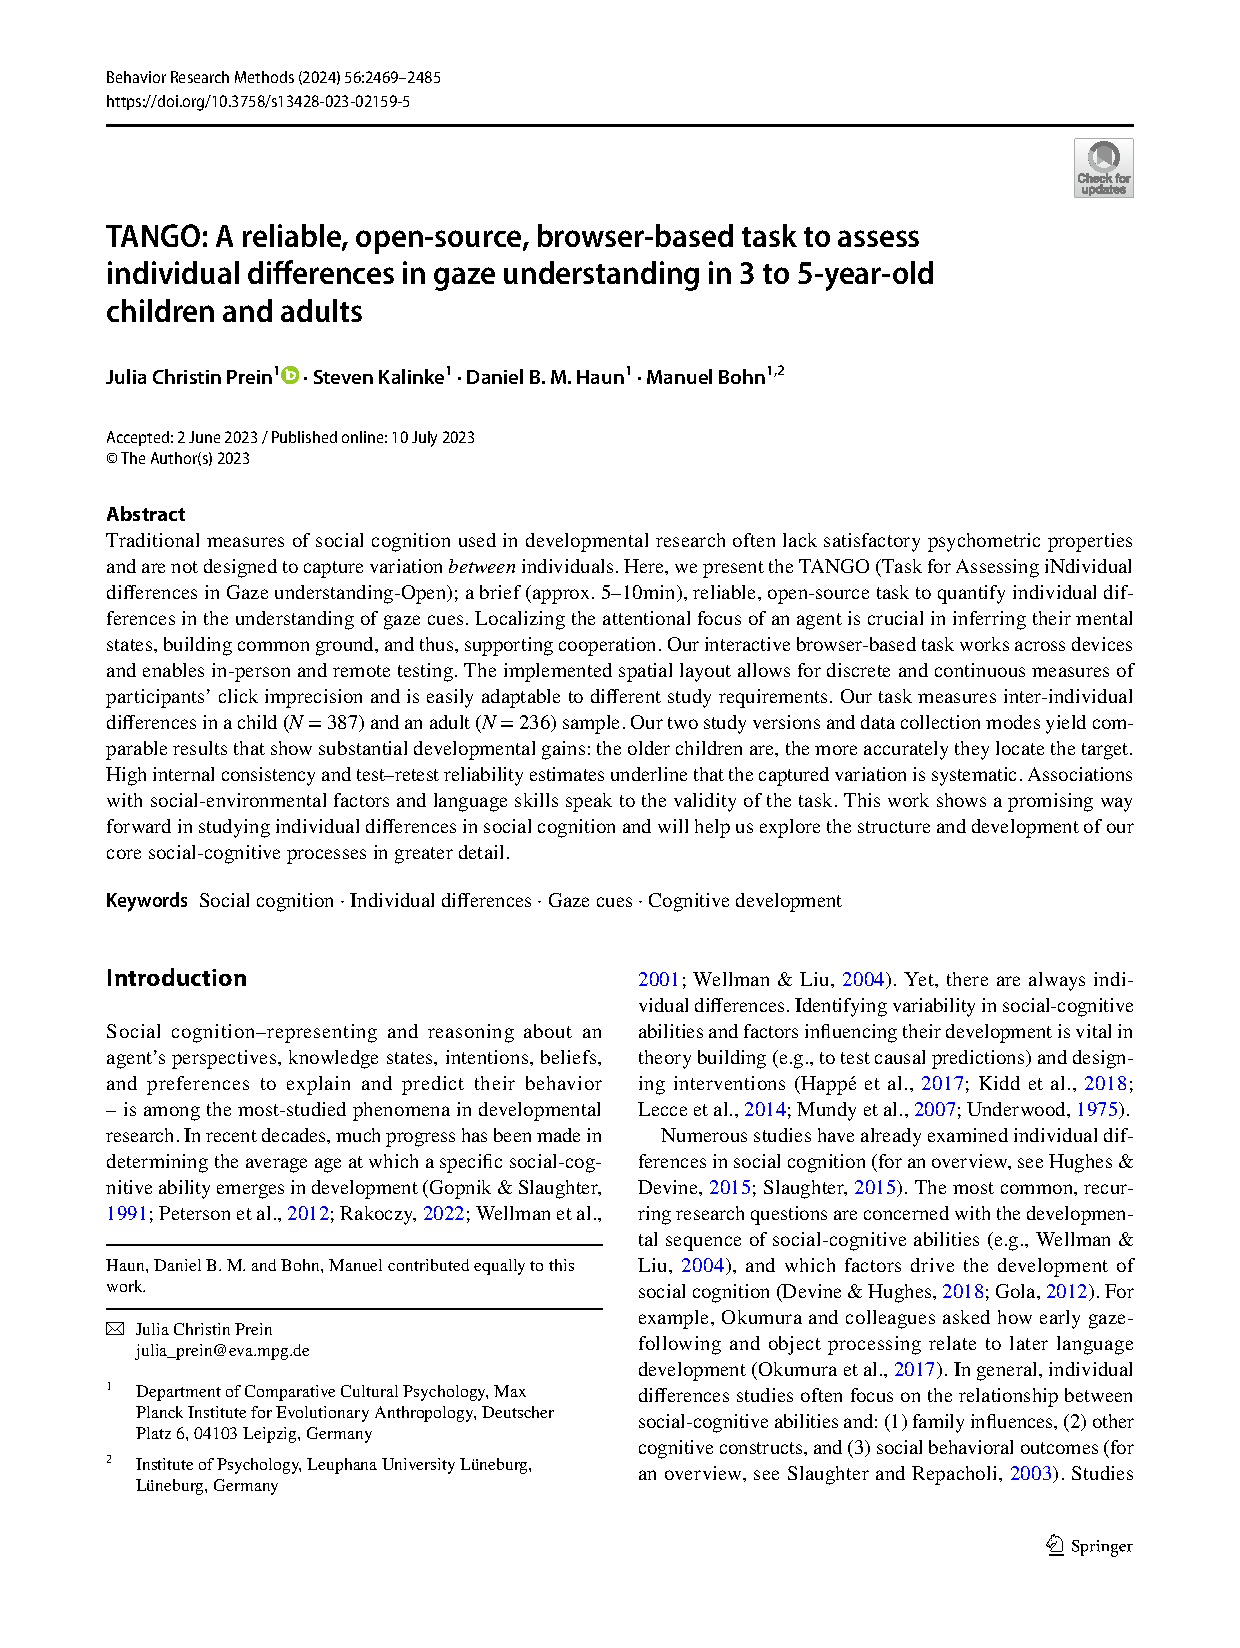
\includepdf[pages={1}, scale=0.85, offset=0 -1cm, pagecommand={}]{../papers/studyI.pdf}
\end{minipage}

\includepdf[pages={2-}, scale=0.85, pagecommand={}]{../papers/studyI.pdf}

\newpage

\section*{Study II}\label{studyII}
\addcontentsline{toc}{section}{Study II}

\begin{minipage}{\textwidth}
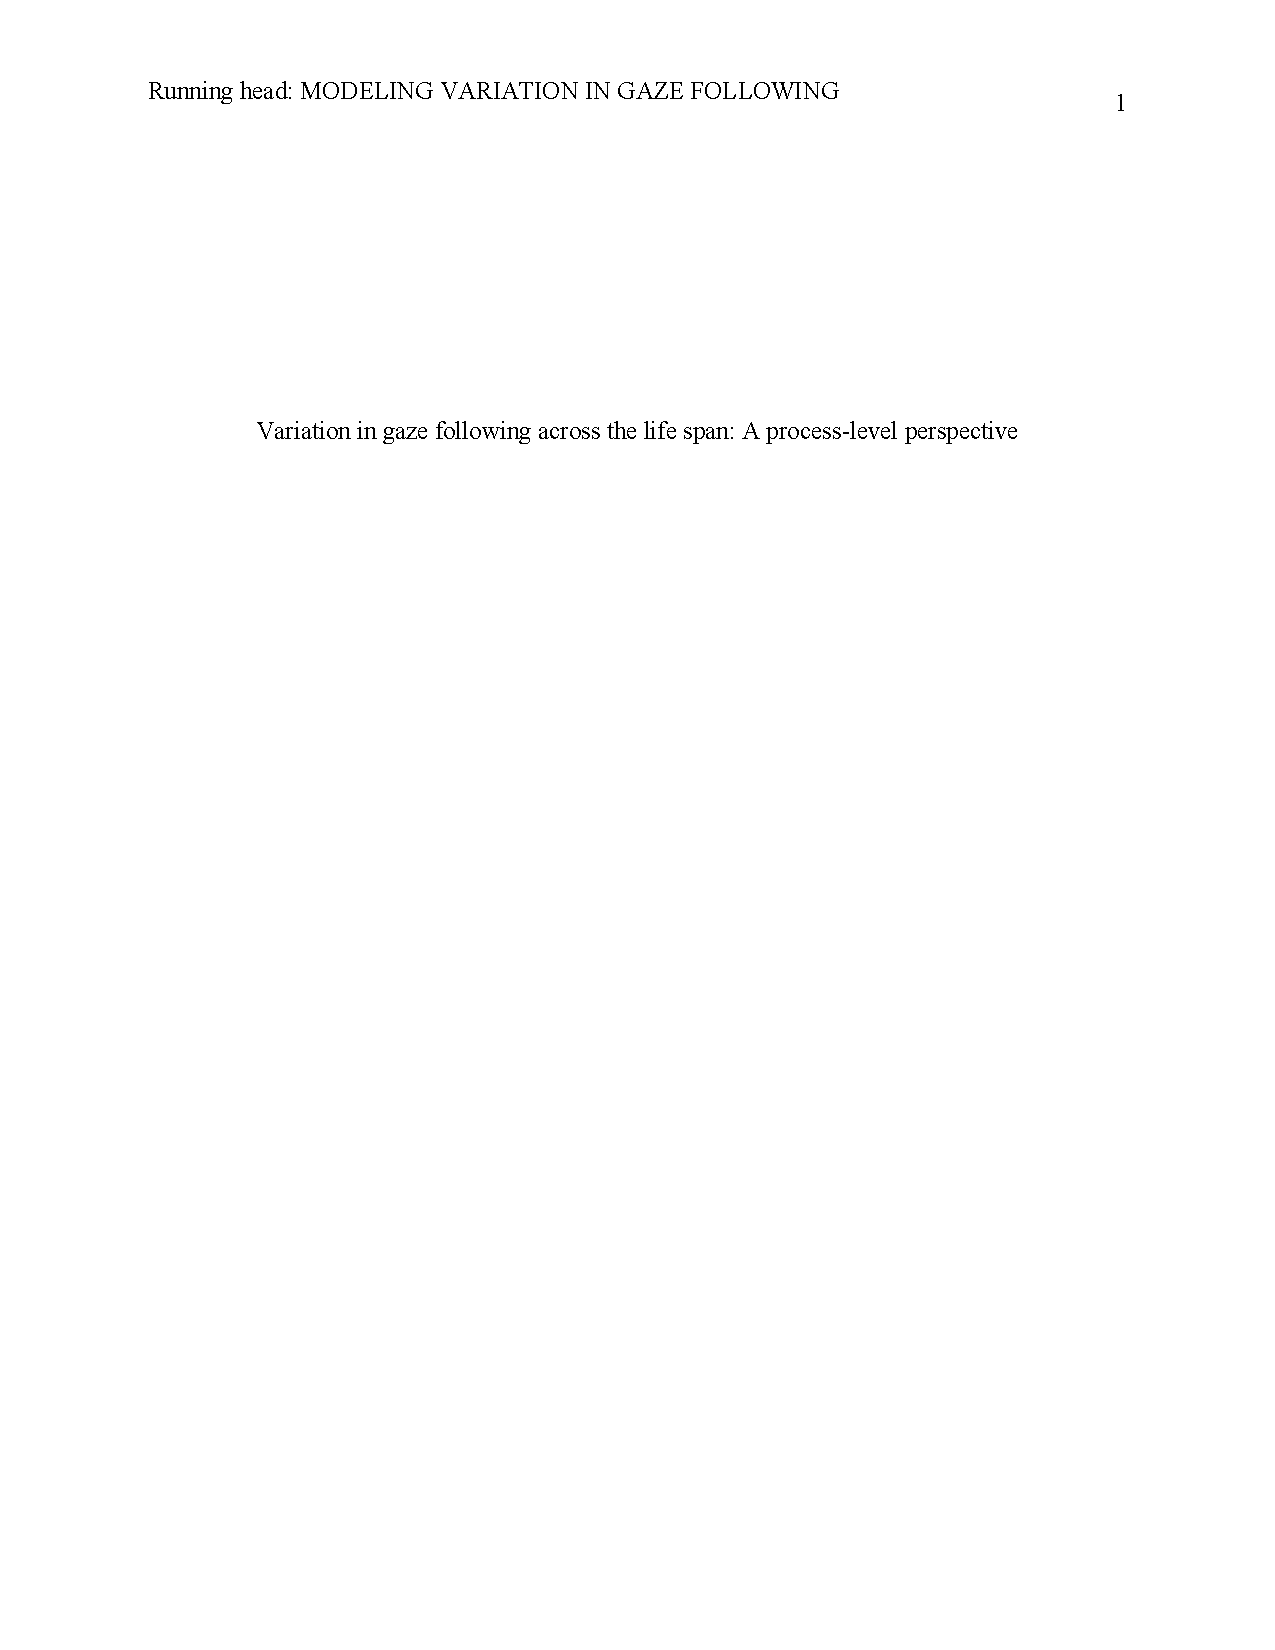
\includepdf[pages={1}, scale=0.85, offset=0 -1cm, pagecommand={}]{../papers/studyII.pdf}
\end{minipage}

\includepdf[pages={2-}, scale=0.85, pagecommand={}]{../papers/studyII.pdf}

\newpage

\section*{Study III}\label{studyIII}
\addcontentsline{toc}{section}{Study III}

\begin{minipage}{\textwidth}
\includepdf[pages={1}, scale=0.85, offset=0 -1cm, pagecommand={}]{../papers/studyIII.pdf}
\end{minipage}

\includepdf[pages={2-}, scale=0.85, pagecommand={}]{../papers/studyIII.pdf}

\newpage

\section*{Study IV}\label{studyIV}
\addcontentsline{toc}{section}{Study IV}

\begin{minipage}{\textwidth}
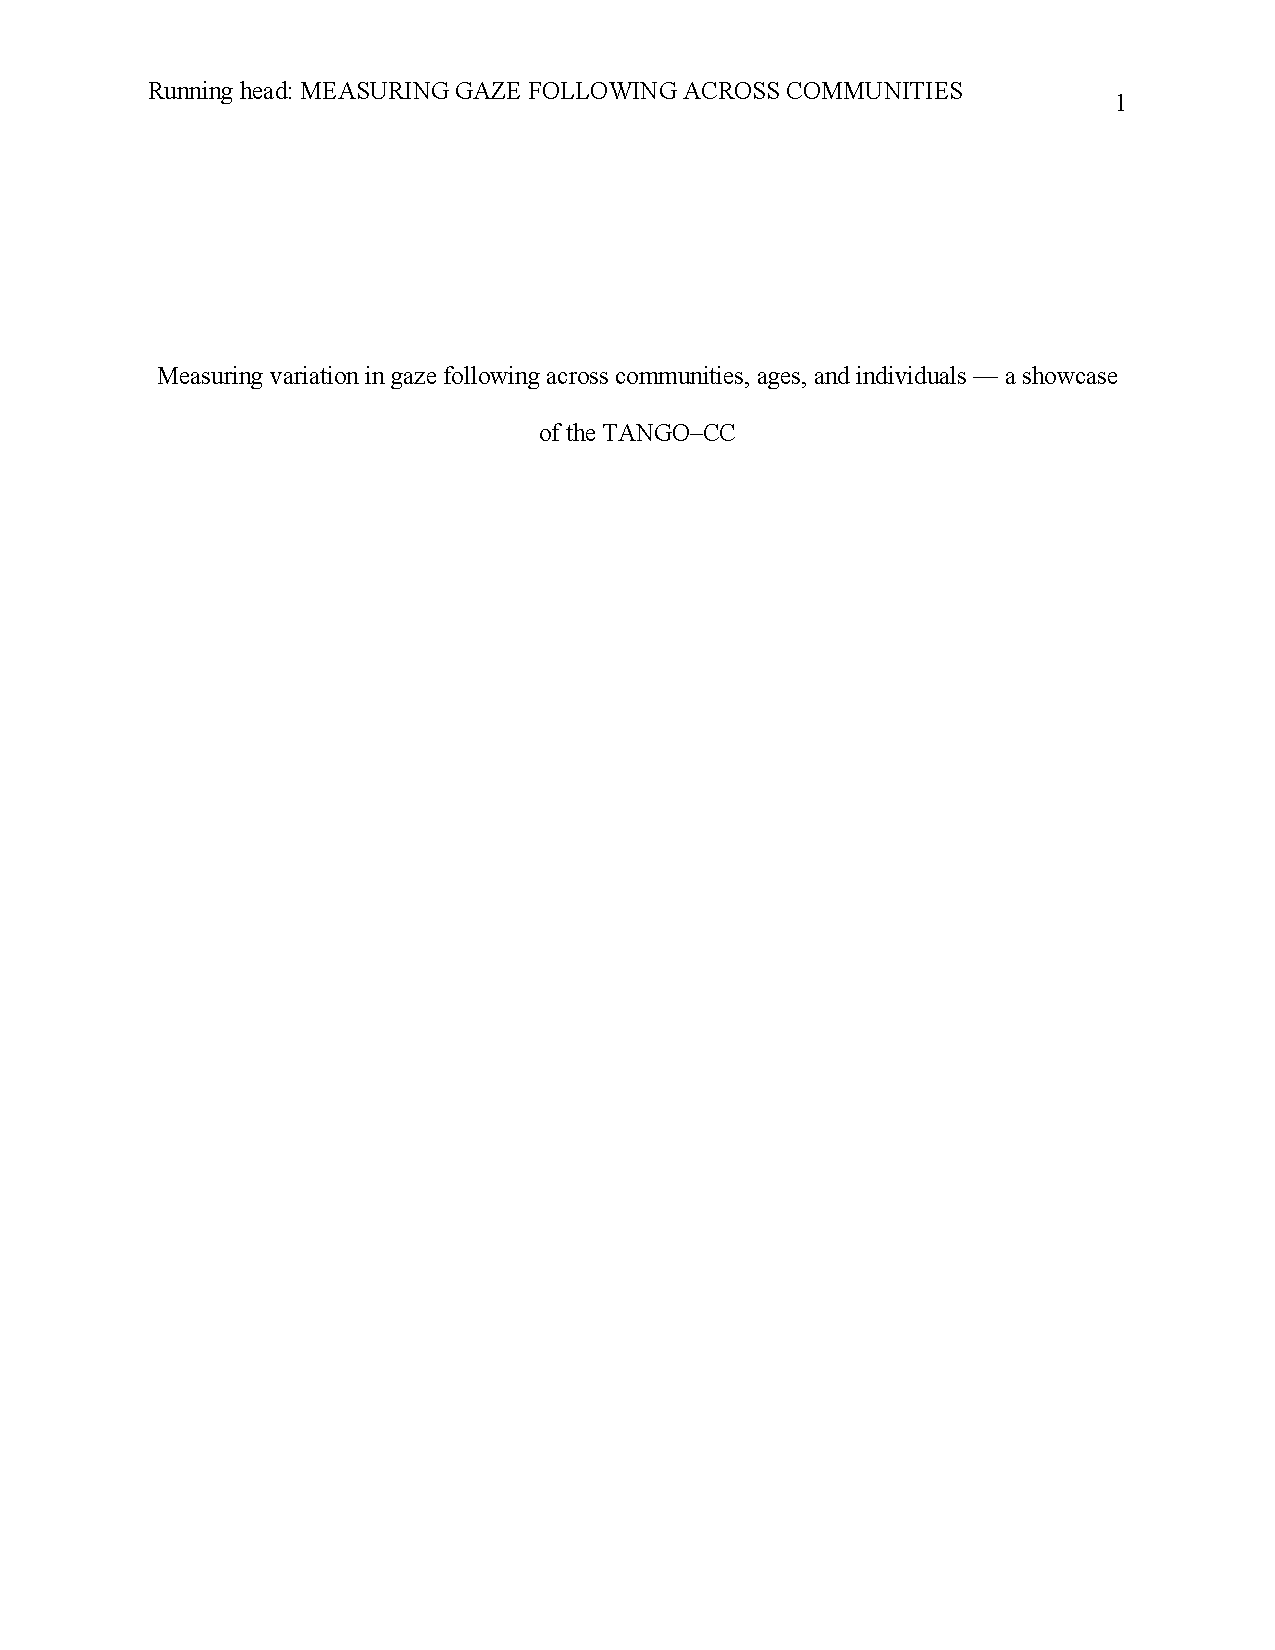
\includepdf[pages={1}, scale=0.85, offset=0 -1cm, pagecommand={}]{../papers/studyIV.pdf}
\end{minipage}

\includepdf[pages={2-}, scale=0.85, pagecommand={}]{../papers/studyIV.pdf}

\chapter*{Appendix B --- Further Publications}\label{appendixB}
\addcontentsline{toc}{chapter}{Appendix B --- Further Publications}

The following Appendix B contains other publications of side projects that were written in the context of the dissertation but not included in the main text, with their respective abstracts.

\section*{Action anticipation based on an agent's epistemic state in toddlers and adults}\label{manybabies}
\addcontentsline{toc}{section}{Action anticipation based on an agent's epistemic state in toddlers and adults}

\textbf{Citation:} Schuwerk, T., Kampis, D., Baillargeon, R., Biro, S., Bohn, M., Byers-Heinlein, K., Dörrenberg, S., Fisher, C., Franchin, L., Fulcher, T., Garbisch, I., Geraci, A., Grosse Wiesmann, C., Hamlin, K., Haun, D. B. M., Hepach, R., Hunnius, S., Hyde, D. C., Karman, P., \ldots, Prein, J., \ldots{} Rakoczy, H. (2021). \emph{Action anticipation based on an agent's epistemic state in toddlers and adults. Child Development} {[}In-Principle Acceptance of Registered Report Stage 1: Study Design{]}. PsyArXiv. \mbox{\url{https://doi.org/10.31234/osf.io/x4jbm}}

\textbf{Abstract:} Do toddlers and adults engage in spontaneous Theory of Mind (ToM)? Evidence from anticipatory looking (AL) studies suggests that they do. But a growing body of failed replication studies raised questions about the paradigm's suitability. In this multi-lab collaboration, we test the robustness of spontaneous ToM measures. We examine whether 18- to 27-month-olds' and adults' anticipatory looks distinguish between two basic forms of an agent's epistemic states: knowledge and ignorance. In toddlers {[}ANTICIPATED n = 520 50\% FEMALE{]} and adults {[}ANTICIPATED n = 408, 50\% FEMALE{]} from diverse ethnic backgrounds, we found {[}SUPPORT/NO SUPPORT{]} for epistemic state-based action anticipation. Future research can probe whether this conclusion extends to more complex kinds of epistemic states, such as true and false beliefs.

\emph{Please note that this abstract was written for the Registered Report and does not entail results yet. Text in square brackets indicates placeholder text to be filled in after data collection.}

\newpage

\section*{PREVIC: An adaptive parent report measure of expressive vocabulary in children between 3 and 8 years of age}\label{previc}
\addcontentsline{toc}{section}{PREVIC: An adaptive parent report measure of expressive vocabulary in children between 3 and 8 years of age}

\textbf{Citation:} Bohn, M., Prein, J. C., Engicht, J., Haun, D., Gagarina, N., \& Koch, T. (2023). \emph{PREVIC: An adaptive parent report measure of expressive vocabulary in children between 3 and 8 years of age.} {[}Manuscript submitted for publication{]}. PsyArXiv. \mbox{\url{https://doi.org/10.31234/osf.io/hvncp}}

\textbf{Abstract:} Parent report measures have proven to be a valuable research tool to study early language development. Caregivers are given a list of words and are asked which of them their child has already used. However, most available measures are not suited for children beyond infancy, come with substantial licensing costs or lack a clear psychometric foundation. Here we present the PREVIC (Parent Report of Expressive Vocabulary in Children), an open access, high quality vocabulary checklist for German-speaking children between three and eight years of age. The PREVIC was constructed leveraging the advantages of Item Response Theory: we designed a large initial item pool of 379 words and collected data from N = 1190 caregivers of children between three and eight years of age. Based on this data, we computed a range of fit indices for each item (word) and used an automated item selection algorithm to compile a final pool that contains items that a) vary in difficulty and b) fit the Rasch (one-parameter logistic) model. The resulting task is highly reliable and shows convergent validity. The IRT-based construction allowed us to design an adaptive version of the task, which substantially reduces the duration of the task while retaining measurement precision. The task -- including the adaptive version -- was implemented as a website and is freely accessible online (\mbox{\url{https://ccp-odc.eva.mpg.de/previc-demo/}}). The PREVIC fills an important gap in the toolkit of researchers interested in language development and provides an ideal starting point for the development of converging measures in other languages.

\newpage

\section*{oREV: An item response theory-based open receptive vocabulary task for 3- to 8-year-old children}\label{orev}
\addcontentsline{toc}{section}{oREV: An item response theory-based open receptive vocabulary task for 3- to 8-year-old children}

\textbf{Citation:} Bohn, M.*, Prein, J.*, Koch, T., Bee, R. M., Delikaya, B., Haun, D., \& Gagarina, N. (2024). oREV: An item response theory-based open receptive vocabulary task for 3- to 8-year-old children. \emph{Behavior Research Methods, 56}(3), 2595--2605. \mbox{\url{https://doi.org/10.3758/s13428-023-02169-3}}

\textbf{Abstract:} Individual differences in early language abilities are an important predictor of later life outcomes. High-quality, easy-access measures of language abilities are rare, especially in the preschool and primary school years. The present study describes the construction of a new receptive vocabulary task for children between 3 and 8 years of age. The task was implemented as a browser-based web application, allowing for both in-person and remote data collection via the internet. Based on data from N = 581 German-speaking children, we estimated the psychometric properties of each item in a larger initial item pool via item response modeling. We then applied an automated item selection procedure to select an optimal subset of items based on item difficulty and discrimination. The so-constructed task has 22 items and shows excellent psychometric properties with respect to reliability, stability, and convergent and discriminant validity. The construction, implementation, and item selection process described here makes it easy to extend the task or adapt it to different languages. All materials and code are freely accessible to interested researchers. The task can be used via the following website: \mbox{\url{https://ccp-odc.eva.mpg.de/orev-demo}}.

\newpage

\section*{Validation of an open source, remote web-based eye-tracking method (WebGazer) for research in early childhood}\label{manywebcams}
\addcontentsline{toc}{section}{Validation of an open source, remote web-based eye-tracking method (WebGazer) for research in early childhood}

\textbf{Citation:} Steffan, A., Zimmer, L., Arias-Trejo, N., Bohn, M., Dal Ben, R., Flores-Coronado, M. A., Franchin, L., Garbisch, I., Grosse Wiesmann, C., Hamlin, J. K., Havron, N., Hay, J. F., Hermansen, T. K., Jakobsen, K. V., Kalinke, S., Ko, E.-S., Kulke, L., Mayor, J., Meristo, M., \ldots, Prein, J., \ldots, Schuwerk, T. (2024). Validation of an open source, remote web-based eye-tracking method (WebGazer) for research in early childhood. \emph{Infancy, 29}(1), 31--55. \mbox{\url{https://doi.org/10.1111/infa.12564}}

\textbf{Abstract:} Measuring eye movements remotely via the participant's webcam promises to be an attractive methodological addition to in-person eye-tracking in the lab. However, there is a lack of systematic research comparing remote web-based eye-tracking with in-lab eye-tracking in young children. We report a multi-lab study that compared these two measures in an anticipatory looking task with toddlers using WebGazer.js and jsPsych. Results of our remotely tested sample of 18-27-month-old toddlers (N = 125) revealed that web-based eye-tracking successfully captured goal-based action predictions, although the proportion of the goal-directed anticipatory looking was lower compared to the in-lab sample (N = 70). As expected, attrition rate was substantially higher in the web-based (42\%) than the in-lab sample (10\%). Excluding trials based on visual inspection of the match of time-locked gaze coordinates and the participant's webcam video overlayed on the stimuli was an important preprocessing step to reduce noise in the data. We discuss the use of this remote web-based method in comparison with other current methodological innovations. Our study demonstrates that remote web-based eye-tracking can be a useful tool for testing toddlers, facilitating recruitment of larger and more diverse samples; a caveat to consider is the larger drop-out rate.

\chapter*{Appendix C --- Social Cognition Survey}\label{appendixC}
\addcontentsline{toc}{chapter}{Appendix C --- Social Cognition Survey}

In Autumn/Winter 2020, we conducted a short online expert survey on defining social cognition, as reported in the Introduction. Below you find the full survey, including the questions and the answers of the experts.

\begin{minipage}{\textwidth}
\includepdf[pages={1}, scale=0.85, offset=0 -1cm, pagecommand={}]{../supplements/social_cognition_survey.pdf}
\end{minipage}

\includepdf[pages={2-}, scale=0.85, pagecommand={}]{../supplements/social_cognition_survey.pdf}

\newpage

\chapter*{Selbstständigkeitserklärung}\label{selbststaendigkeit}
\addcontentsline{toc}{chapter}{Selbstständigkeitserklärung}

Julia Christin Prein\\
{[}Straße Hausnummer{]}\\
{[}PLZ Ort{]}\\
{[}Telefon{]}\\
{[}Email{]}\\

Hiermit erkläre ich, dass ich mich noch keiner Doktorprüfung unterzogen oder mich um Zulassung zu einer solchen beworben habe.

Ich versichere, dass die Dissertation \emph{Rethinking Variation in Social Cognition: Gaze Following across Individuals, Ages, and Communities} in der gegenwärtigen oder einer anderen Fassung noch keiner anderen Hochschule zur Begutachtung vorgelegen hat.

Ich versichere an Eides statt, dass ich die eingereichte Dissertation \emph{Rethinking Variation in Social Cognition: Gaze Following across Individuals, Ages, and Communities} selbstständig und ohne zulässige fremde Hilfe verfasst habe. Anderer als der von mir angegebenen Hilfsmittel und Schriften habe ich mich nicht bedient. Alle wörtlich oder sinngemäß anderen Schriften entnommenen Stellen habe ich kenntlich gemacht. Über die strafrechtlichen Folgen gemäß § 156 Strafgesetzbuch wurde ich in Kenntnis gesetzt.

~

Hamburg, {[}Datum{]}

~

{[}Unterschrift{]}

\end{document}
